% ═══════════════════════════════════════════════════════════════════════════════
%  RAPPORT DE PROJET DE FIN D'ÉTUDES
%  EduAI — Assistant Pédagogique Intelligent (SaaS)
%  EL Mehdi HACHAMI · Bachelor Ingénierie Informatique en IA & Sciences des Données
%  École Supérieure de Technologie — Essaouira · Université Cadi Ayyad
%  Année universitaire 2025/2026
% ═══════════════════════════════════════════════════════════════════════════════
\documentclass[12pt, a4paper, oneside]{report}

% ── Encodage et langue ─────────────────────────────────────────────────────
\usepackage[utf8]{inputenc}
\usepackage[T1]{fontenc}
\usepackage[french]{babel}
\usepackage{lmodern}
\usepackage[final]{microtype}

% ── Mise en page ───────────────────────────────────────────────────────────
\usepackage[top=2.5cm, bottom=2.5cm, left=3cm, right=2.5cm, headheight=14.2pt]{geometry}
\usepackage{setspace}
\onehalfspacing
\usepackage{fancyhdr}
\usepackage{truncate}
\usepackage{titlesec}
\usepackage{titletoc}

% ── Graphiques et couleurs ─────────────────────────────────────────────────
\usepackage{graphicx}
\usepackage[table,xcdraw]{xcolor}
\usepackage{float}
\usepackage{subcaption}

% ── Tableaux ───────────────────────────────────────────────────────────────
\usepackage{array}
\usepackage{booktabs}
\usepackage{longtable}
\usepackage{multirow}
\usepackage{tabularx}

% ── Listes et énumérations ────────────────────────────────────────────────
\usepackage{enumitem}

% ── Liens et références ───────────────────────────────────────────────────
\usepackage[hidelinks, colorlinks=true, linkcolor=black, citecolor=blue, urlcolor=blue]{hyperref}
\usepackage{url}

% ── Code source ────────────────────────────────────────────────────────────
\usepackage{listings}
\usepackage{minted}

% ── Divers ─────────────────────────────────────────────────────────────────
\usepackage{amsmath}
\usepackage{amssymb}
\usepackage{pdfpages}
\usepackage{appendix}

% ── Typographie (justification sans coupure en fin de ligne) ────────────────
\tolerance=1000
\setlength{\emergencystretch}{3em}
\hyphenpenalty=10000
\exhyphenpenalty=10000

% ── Couleurs personnalisées ────────────────────────────────────────────────
\definecolor{eduai-primary}{HTML}{2563EB}
\definecolor{eduai-dark}{HTML}{1E293B}
\definecolor{este-brown}{HTML}{8B1A1A}
\definecolor{gray-light}{HTML}{F8FAFC}
\definecolor{table-row-alt}{HTML}{EFF6FF}

% ── Design professionnel des tableaux ─────────────────────────────────────
\setlength{\extrarowheight}{3pt}
\renewcommand{\arraystretch}{1.35}
\arrayrulecolor{eduai-primary}
% Entête de colonne : fond bleu + texte blanc gras
\newcommand{\thead}[1]{\textcolor{white}{\textbf{#1}}}

% ── En-têtes et pieds de page ──────────────────────────────────────────────
\pagestyle{fancy}
\fancyhf{}
\fancyhead[L]{\small\truncate{0.58\textwidth}{\leftmark}}
\fancyhead[R]{\small EduAI — Rapport PFE}
\fancyfoot[C]{\thepage}
\renewcommand{\headrulewidth}{0.4pt}
\renewcommand{\footrulewidth}{0.2pt}

% ── Style des chapitres ────────────────────────────────────────────────────
\titleformat{\chapter}[display]
  {\normalfont\huge\bfseries\color{eduai-dark}}
  {\chaptertitlename\ \thechapter}{20pt}{\Huge}
\titlespacing*{\chapter}{0pt}{-20pt}{30pt}

% ── Listings config ────────────────────────────────────────────────────────
\lstset{
  basicstyle=\ttfamily\small,
  breaklines=true,
  frame=single,
  backgroundcolor=\color{gray-light},
  keywordstyle=\color{eduai-primary}\bfseries,
  commentstyle=\color{gray},
  stringstyle=\color{green!50!black},
}

% ══════════════════════════════════════════════════════════════════════════════
\begin{document}

% ── PAGE DE GARDE ──────────────────────────────────────────────────────────
\begin{titlepage}
\begin{center}

% Logo ESTE

\includegraphics[width=10cm, trim=112 90 140 75, clip]{figures/logo_este.png}

\vspace{0.5cm}
{\large \textbf{Université Cadi Ayyad}}\\[0.2cm]
{\large École Supérieure de Technologie — Essaouira}\\[0.3cm]
{\normalsize Filière : Bachelor en Ingénierie Informatique en Intelligence Artificielle et Sciences des Données}

\vspace{1.2cm}
\rule{\textwidth}{1.5pt}\\[0.4cm]
{\fontsize{22}{26}\selectfont \textbf{Rapport de Projet de Fin d'Études}}\\[0.3cm]
\rule{\textwidth}{1.5pt}

\vspace{0.8cm}
{\fontsize{18}{22}\selectfont \textcolor{eduai-primary}{\textbf{EduAI — Assistant Pédagogique Intelligent}}}\\[0.3cm]
{\large Plateforme SaaS d'apprentissage augmenté par l'Intelligence Artificielle}

\vspace{1.5cm}

\begin{minipage}[t]{0.45\textwidth}
\textbf{Réalisé par :}\\[0.2cm]
EL Mehdi HACHAMI
\end{minipage}
\hfill
\begin{minipage}[t]{0.45\textwidth}
\textbf{Encadré par :}\\[0.2cm]
Pr. El Mahdi ERRAJI
\end{minipage}

\vspace{1cm}

\begin{minipage}[t]{0.45\textwidth}
\textbf{Entreprise :}\\[0.2cm]
2Pi eLearning SARL
\end{minipage}
\hfill
\begin{minipage}[t]{0.45\textwidth}
\textbf{Poste :}\\[0.2cm]
Développeur Full-stack et Responsable des Opérations
\end{minipage}

\vfill
{\large \textbf{Année universitaire : 2025 / 2026}}

\end{center}
\end{titlepage}

% ── PAGES LIMINAIRES ──────────────────────────────────────────────────────
\hypersetup{pageanchor=false}
\pagenumbering{roman}

% Dédicace
\chapter*{Dédicace}
\addcontentsline{toc}{chapter}{Dédicace}
\vspace{2cm}
\begin{center}
\textit{À mes chers parents,\\
À ma famille,\\
À tous ceux qui m'ont soutenu tout au long de ce parcours.}
\end{center}
\newpage

% Remerciements
\chapter*{Remerciements}
\addcontentsline{toc}{chapter}{Remerciements}

Je souhaite remercier toutes les personnes qui m'ont aidé durant ce projet de fin d'études.

Tout d'abord, je remercie mon encadrant, \textbf{Professeur El Mahdi ERRAJI}, pour ses conseils, son suivi et ses orientations tout au long de ce travail.

Je remercie aussi l'entreprise \textbf{2Pi eLearning SARL}, où je travaille comme Développeur Full-stack et Responsable des Opérations, pour avoir mis à ma disposition l'infrastructure nécessaire au déploiement de la plateforme.

Je tiens également à remercier les enseignants de la filière \textbf{Bachelor en Ingénierie Informatique en Intelligence Artificielle et Sciences des Données} à l'\textbf{École Supérieure de Technologie d'Essaouira} pour la formation de qualité que j'ai reçue.

Enfin, merci aux membres du jury d'avoir accepté d'évaluer ce travail.

\newpage

% Résumé
\chapter*{Résumé}
\addcontentsline{toc}{chapter}{Résumé}

Le présent rapport décrit la conception et la réalisation d'\textbf{EduAI}, une plateforme SaaS (\textit{Software as a Service}) d'assistance pédagogique basée sur l'Intelligence Artificielle. Ce projet, réalisé de manière entièrement individuelle sous l'encadrement de \textbf{Pr. El Mahdi ERRAJI}, vise à répondre à une problématique concrète rencontrée par de nombreux étudiants de l'enseignement supérieur marocain : la difficulté à assimiler efficacement les cours volumineux distribués sous format PDF. L'entreprise \textbf{2Pi eLearning SARL}, au sein de laquelle l'auteur exerce comme Développeur Full-stack et Responsable des Opérations, a mis à disposition l'infrastructure de déploiement (Portainer).

La plateforme EduAI propose six outils d'apprentissage complémentaires : un module de résumé pédagogique automatique par chapitre, un système de questions-réponses conversationnel fondé sur l'approche RAG (\textit{Retrieval-Augmented Generation}), un générateur de quiz adaptatifs, des flashcards intégrant l'algorithme de répétition espacée SM-2, des cartes mentales interactives, ainsi qu'un mode examen chronométré avec notation automatique. L'ensemble de ces fonctionnalités est généré automatiquement à partir du contenu spécifique de chaque cours uploadé.

L'architecture technique repose sur un backend \textbf{FastAPI} (Python), un frontend \textbf{Next.js} (React/TypeScript), une base de données \textbf{MongoDB}, et des modèles d'Intelligence Artificielle (Llama 3.3 70B via Groq, embeddings multilingues MiniLM, FAISS) orchestrés au sein d'un pipeline RAG complet.

\vspace{0.5cm}
\textbf{Mots-clés :} Intelligence Artificielle, EdTech, SaaS, NLP, RAG, LLM, FastAPI, Next.js, MongoDB, apprentissage adaptatif.

\newpage

% Tables
\addcontentsline{toc}{chapter}{Table des matières}
\tableofcontents
\newpage

% Liste des figures
\listoffigures
\markboth{Table des figures}{Table des figures}
\addcontentsline{toc}{chapter}{Table des figures}
\newpage

% Liste des tableaux
\listoftables
\markboth{Liste des tableaux}{Liste des tableaux}
\addcontentsline{toc}{chapter}{Liste des tableaux}
\newpage

% Liste des abréviations
\chapter*{Liste des abréviations}
\markboth{Liste des abréviations}{Liste des abréviations}
\addcontentsline{toc}{chapter}{Liste des abréviations}
\begin{longtable}{@{}ll@{}}
\toprule
\rowcolor{eduai-primary}
\thead{Abréviation} & \thead{Signification} \\
\midrule
\endfirsthead
\toprule
\rowcolor{eduai-primary}
\thead{Abréviation} & \thead{Signification} \\
\midrule
\endhead
AI / IA & Artificial Intelligence / Intelligence Artificielle \\
API & Application Programming Interface \\
CORS & Cross-Origin Resource Sharing \\
CRUD & Create, Read, Update, Delete \\
CSS & Cascading Style Sheets \\
FAISS & Facebook AI Similarity Search \\
JWT & JSON Web Token \\
LLM & Large Language Model \\
MLD & Modèle Logique de Données \\
NLP & Natural Language Processing \\
PDF & Portable Document Format \\
RAG & Retrieval-Augmented Generation \\
REST & Representational State Transfer \\
SaaS & Software as a Service \\
SM-2 & SuperMemo Algorithm 2 \\
UML & Unified Modeling Language \\
UUID & Universally Unique Identifier \\
\bottomrule
\end{longtable}
\newpage

% ── CORPS DU RAPPORT ──────────────────────────────────────────────────────
\hypersetup{pageanchor=true}
\pagenumbering{arabic}
\setcounter{page}{1}

% Introduction générale
\chapter*{Introduction générale}
\markboth{Introduction générale}{Introduction générale}
\addcontentsline{toc}{chapter}{Introduction générale}
% ══════════════════════════════════════════════════════════════════════════════
%  INTRODUCTION GÉNÉRALE
% ══════════════════════════════════════════════════════════════════════════════

Depuis quelques années, le numérique a considérablement transformé les méthodes d'enseignement et d'apprentissage. Au Maroc, cette évolution est portée par la Vision Stratégique 2015-2030 et le programme Maroc Digital 2030, qui accordent une place importante à la modernisation du système éducatif. Malgré ces avancées, les étudiants de l'enseignement supérieur continuent de recevoir l'essentiel de leurs cours sous format PDF, un format qui reste difficile à exploiter sans outils interactifs adaptés.

C'est dans ce contexte qu'a été conçu \textbf{EduAI}, une plateforme SaaS (\textit{Software as a Service}) qui s'appuie sur l'Intelligence Artificielle, et plus précisément sur le Traitement Automatique du Langage Naturel (NLP) et les grands modèles de langage (LLM), pour permettre aux étudiants de transformer leurs cours PDF en supports d'apprentissage interactifs.

Ce rapport présente le travail réalisé dans le cadre du Projet de Fin d'Études de la filière Bachelor en Ingénierie Informatique en Intelligence Artificielle et Sciences des Données, à l'École Supérieure de Technologie d'Essaouira (Université Cadi Ayyad). L'idée du projet est partie d'un constat simple : beaucoup d'étudiants peinent à réviser efficacement à partir de cours PDF souvent longs et denses.

\textbf{EduAI} est un projet personnel que j'ai réalisé seul, sous l'encadrement de \textbf{Pr. El Mahdi ERRAJI}. En parallèle de mes études, je travaille comme Développeur Full-stack et Responsable des Opérations chez \textbf{2Pi eLearning SARL}, qui a bien voulu mettre à disposition un espace sur son infrastructure Portainer pour héberger la plateforme.

\vspace{0.5cm}
Le présent rapport est organisé en cinq chapitres :

\begin{enumerate}[label=\textbf{Chapitre~\arabic* :}]
  \item \textbf{Contexte général et problématique} — Présentation de l'organisme d'accueil, analyse du contexte éducatif marocain, formulation de la problématique et étude critique de l'existant.
  \item \textbf{Analyse et spécification des besoins} — Identification des acteurs, spécification des besoins fonctionnels et non-fonctionnels, et modélisation UML des cas d'utilisation.
  \item \textbf{Conception} — Architecture globale du système, conception des pipelines NLP/IA, modélisation de la base de données et conception de l'API REST.
  \item \textbf{Réalisation} — Environnement technique, choix technologiques, présentation des modules implémentés et validation par les tests.
  \item \textbf{Déploiement, modèle économique et perspectives} — Stratégie de déploiement conteneurisé, modèle SaaS freemium, projections financières et axes d'évolution.
\end{enumerate}

Les diagrammes UML et les captures d'écran des interfaces sont regroupés en annexes.


% Chapitre 1
\chapter{Contexte général et problématique}
% ══════════════════════════════════════════════════════════════════════════════
%  CHAPITRE 1 — CONTEXTE GÉNÉRAL ET PROBLÉMATIQUE
% ══════════════════════════════════════════════════════════════════════════════

\section{Présentation de l'organisme d'accueil}

\subsection{Fiche signalétique}

\begin{table}[H]
\centering
\begin{tabularx}{\textwidth}{lX}
\toprule
\rowcolor{table-row-alt}
\textbf{Raison sociale}      & 2Pi eLearning SARL \\
\midrule
\textbf{Secteur d'activité}  & EdTech — Technologies éducatives numériques \\
\textbf{Date de création}    & 2022 \\
\textbf{Effectif}            & Équipe pluridisciplinaire (développeurs, designers, experts pédagogiques) \\
\textbf{Mission}             & Rendre l'apprentissage plus interactif, engageant et accessible \\
\textbf{Domaine}             & Solutions e-learning, plateformes pédagogiques intelligentes \\
\bottomrule
\end{tabularx}
\caption{Fiche signalétique de 2Pi eLearning SARL}
\label{tab:fiche-entreprise}
\end{table}

\subsection{Présentation de l'entreprise}

\textbf{2Pi eLearning SARL} est une entreprise marocaine fondée en 2022, spécialisée dans le développement de solutions éducatives numériques. Elle intervient dans le secteur EdTech avec pour objectif de proposer des outils d'apprentissage plus interactifs et accessibles.

L'équipe est composée de développeurs, de designers et de spécialistes en pédagogie. L'entreprise développe principalement des plateformes d'apprentissage en ligne, en intégrant des technologies comme l'Intelligence Artificielle et le Traitement Automatique du Langage Naturel.

Dans le cadre de ce projet, 2Pi eLearning a mis à disposition un espace sur son infrastructure \textbf{Portainer}, ce qui a permis d'héberger EduAI dans un environnement de production.

\subsection{Contexte du projet}

L'idée de ce projet vient d'un problème que j'ai moi-même rencontré en tant qu'étudiant : la difficulté de réviser à partir de cours PDF souvent très longs. \textbf{EduAI} est donc un projet personnel, conçu pour apporter une réponse concrète à ce besoin.

J'ai réalisé l'ensemble du projet seul, de la conception au déploiement, sous l'encadrement de \textbf{Pr. El Mahdi ERRAJI}. En parallèle de mes études, je travaille comme \textbf{Développeur Full-stack et Responsable des Opérations} chez \textbf{2Pi eLearning SARL}, qui a fourni l'infrastructure de déploiement.

% ──────────────────────────────────────────────────────────────────────────────
\section{Contexte général}

\subsection{Le paysage éducatif au Maroc}

Le système éducatif marocain connaît actuellement plusieurs évolutions importantes :

\begin{itemize}
  \item \textbf{Vision Stratégique 2015-2030 :} le Maroc a engagé une réforme globale de son système éducatif, avec un accent particulier sur la digitalisation et l'innovation pédagogique.
  \item \textbf{Programme Maroc Digital 2030 :} cette stratégie nationale accélère la transition numérique dans l'ensemble des secteurs, y compris l'éducation.
  \item \textbf{Impact post-pandémique :} la crise sanitaire a révélé les limites de l'enseignement à distance et a accéléré l'adoption de solutions numériques.
  \item \textbf{Démographie jeune :} avec plus d'un million d'étudiants dans l'enseignement supérieur, la demande en outils pédagogiques innovants est considérable.
\end{itemize}

\subsection{La digitalisation de l'enseignement supérieur}

Les universités marocaines ont largement adopté la diffusion de cours sous format numérique (PDF, présentations, documents scannés). Si cette digitalisation répond au problème d'accessibilité physique aux supports, elle engendre de nouveaux défis :

\begin{itemize}
  \item Des documents souvent volumineux (50 à 200 pages par matière et par semestre) ;
  \item Un format intrinsèquement passif, n'encourageant pas l'interaction ;
  \item L'absence d'outils d'auto-évaluation intégrés ;
  \item La difficulté de synthétiser et de mémoriser un grand volume d'informations.
\end{itemize}

% ──────────────────────────────────────────────────────────────────────────────
\section{Problématique}

\subsection{Constat}

L'observation du quotidien académique des étudiants marocains fait apparaître un problème fréquent :

\begin{quote}
\textit{\og De nombreux étudiants reçoivent des cours au format PDF, souvent longs, denses et difficiles à assimiler. Cette surcharge informationnelle engendre des difficultés de compréhension qui se répercutent directement sur les résultats académiques et la réussite des parcours universitaires. \fg{}}
\end{quote}

\subsection{Analyse détaillée}

Les difficultés identifiées couvrent plusieurs aspects :

\begin{table}[H]
\centering
\begin{tabularx}{\textwidth}{lX}
\toprule
\rowcolor{eduai-primary}
\thead{Dimension} & \thead{Description} \\
\midrule
\textbf{Volume}           & Cours PDF de 50 à 200+ pages, avec plusieurs matières en parallèle \\
\textbf{Densité}          & Contenu académique complexe, terminologie spécialisée \\
\textbf{Passivité}        & Format statique ne permettant aucune interaction avec le contenu \\
\textbf{Mémorisation}     & Absence de mécanisme de révision structurée ou de répétition espacée \\
\textbf{Auto-évaluation}  & Aucun outil permettant à l'étudiant de tester ses acquis avant l'examen \\
\textbf{Synthèse}         & Difficulté à identifier et extraire les concepts clés d'un document long \\
\textbf{Visualisation}    & Absence de représentation visuelle des liens entre les concepts \\
\bottomrule
\end{tabularx}
\caption{Dimensions de la problématique étudiante}
\label{tab:problematique}
\end{table}

\subsection{Impact sur la réussite académique}

Ces difficultés s'enchaînent et se renforcent mutuellement :

\begin{enumerate}
  \item L'étudiant reçoit un PDF volumineux $\rightarrow$ découragement face au volume ;
  \item Lecture passive sans interaction $\rightarrow$ faible rétention de l'information ;
  \item Absence de mécanisme de révision $\rightarrow$ oubli rapide (courbe d'Ebbinghaus) ;
  \item Pas d'auto-évaluation $\rightarrow$ fausse confiance ou anxiété ;
  \item Résultat : \textbf{notes insuffisantes} et \textbf{risque d'échec académique}.
\end{enumerate}

\subsection{Formulation de la problématique}

\begin{center}
\fbox{\parbox{0.9\textwidth}{
\textbf{Problématique :} Comment exploiter l'Intelligence Artificielle et le Traitement Automatique du Langage Naturel pour transformer des documents PDF de cours en une expérience d'apprentissage interactive, personnalisée et mesurable, permettant aux étudiants d'améliorer significativement leur compréhension et leur réussite académique ?
}}
\end{center}

% ──────────────────────────────────────────────────────────────────────────────
\section{Étude de l'existant}

\subsection{Solutions existantes sur le marché}

Plusieurs solutions tentent de répondre, partiellement, à cette problématique. Le tableau~\ref{tab:existant} en présente une synthèse comparative :

\begin{table}[H]
\centering
\small
\begin{tabularx}{\textwidth}{lXX}
\toprule
\rowcolor{eduai-primary}
\thead{Solution} & \thead{Fonctionnalités} & \thead{Limites} \\
\midrule
\textbf{ChatGPT / Claude} & Q\&A généraliste, résumé de texte & Non spécialisé pour l'éducation, pas de suivi de progression, risque d'hallucinations hors contexte, pas de quiz structuré \\
\textbf{Quizlet} & Flashcards, quiz basiques & Création manuelle, pas d'IA générative, pas de résumé, pas d'analyse de PDF \\
\textbf{Notion AI} & Résumé, Q\&A sur documents & Pas de quiz, pas de flashcards, pas de mode examen, modèle freemium limité \\
\textbf{Coursera / EdX} & Cours structurés avec quiz & Contenu prédéfini, ne traite pas les PDF personnels de l'étudiant \\
\textbf{SciSpace / Scholarcy} & Résumé d'articles scientifiques & Orienté recherche, pas d'apprentissage interactif, pas de quiz, anglophone \\
\textbf{Anki} & Flashcards avec algorithme SM-2 & Création manuelle fastidieuse, pas de génération automatique, pas de résumé \\
\bottomrule
\end{tabularx}
\caption{Analyse comparative des solutions existantes}
\label{tab:existant}
\end{table}

\subsection{Analyse critique}

En examinant les solutions disponibles sur le marché, on constate plusieurs manques :

\begin{enumerate}[label=\textbf{C\arabic*.}]
  \item \textbf{Fragmentation fonctionnelle :} aucune solution ne propose un écosystème intégré réunissant résumé, Q\&A, quiz, flashcards, carte mentale et examen au sein d'une même plateforme.
  
  \item \textbf{Absence de personnalisation contextuelle :} les outils généralistes (ChatGPT, Claude) ne sont pas ancrés dans le contenu spécifique du cours, ce qui génère des hallucinations et des réponses hors contexte.
  
  \item \textbf{Absence de pipeline RAG :} sans mécanisme de \textit{Retrieval-Augmented Generation}, les réponses ne sont pas fidèles au document source.
  
  \item \textbf{Création manuelle obligatoire :} Quizlet et Anki exigent que l'étudiant crée manuellement ses fiches, ce qui consomme un temps précieux.
  
  \item \textbf{Support multilingue insuffisant :} la majorité des solutions sont optimisées pour l'anglais, sans support natif du français technique utilisé dans les universités marocaines.
  
  \item \textbf{Coût élevé :} les solutions professionnelles sont souvent inadaptées au budget des étudiants marocains.
  
  \item \textbf{Absence de suivi de progression :} aucune plateforme ne combine apprentissage actif et analytique de performance.
\end{enumerate}

% ──────────────────────────────────────────────────────────────────────────────
\section{Solution proposée : EduAI}

\subsection{Vision globale}

\textbf{EduAI} est une plateforme SaaS qui permet à un étudiant d'uploader son cours PDF et d'obtenir automatiquement plusieurs outils d'apprentissage générés par l'IA :

\begin{center}
\fbox{\parbox{0.88\textwidth}{
\centering
\vspace{0.3cm}
\textbf{PDF du cours} $\xrightarrow{\text{Upload}}$ \textbf{Pipeline IA} $\xrightarrow{\text{Génération automatique}}$ 
\begin{itemize}[nosep, leftmargin=*]
  \item[\checkmark] Résumé pédagogique structuré par chapitre
  \item[\checkmark] Chat Q\&A contextuel (RAG)
  \item[\checkmark] Quiz adaptatifs auto-générés
  \item[\checkmark] Flashcards avec répétition espacée (SM-2)
  \item[\checkmark] Carte mentale interactive
  \item[\checkmark] Mode examen chronométré
\end{itemize}
\vspace{0.2cm}
}}
\end{center}

\subsection{Positionnement et différenciation}

EduAI se distingue des outils existants sur plusieurs points :

\begin{table}[H]
\centering
\begin{tabularx}{\textwidth}{lX}
\toprule
\rowcolor{eduai-primary}
\thead{Axe de différenciation} & \thead{Description} \\
\midrule
\textbf{Plateforme intégrée} & Six outils d'apprentissage réunis dans une seule plateforme \\
\textbf{RAG contextuel} & Réponses fidèles au document source, éliminant les hallucinations \\
\textbf{Automatisation complète} & Aucune création manuelle requise : tout est généré par l'IA \\
\textbf{Multilingue natif} & Support du français et de l'arabe via des embeddings multilingues \\
\textbf{Apprentissage adaptatif} & Algorithme SM-2 pour la révision espacée, difficulté progressive \\
\textbf{Accessibilité tarifaire} & Modèle freemium adapté au budget des étudiants marocains \\
\textbf{Suivi de progression} & Statistiques détaillées, activité journalière, taux de réussite \\
\bottomrule
\end{tabularx}
\caption{Axes de différenciation d'EduAI}
\label{tab:differenciation}
\end{table}

\subsection{Objectifs du projet}

Les objectifs de ce PFE se répartissent en trois catégories :

\subsubsection{Objectifs techniques}
\begin{itemize}
  \item Concevoir et implémenter un pipeline RAG complet (extraction, chunking, embeddings, retrieval, génération) ;
  \item Développer une API REST performante et asynchrone avec FastAPI ;
  \item Créer une interface utilisateur moderne et responsive avec Next.js ;
  \item Intégrer des modèles d'IA multilingues (Groq/Llama 3.3 70B, sentence-transformers, CamemBERT) ;
  \item Implémenter l'algorithme de répétition espacée SM-2 pour les flashcards.
\end{itemize}

\subsubsection{Objectifs fonctionnels}
\begin{itemize}
  \item Permettre l'upload et le traitement automatique de cours PDF ;
  \item Générer des résumés pédagogiques structurés par chapitre ;
  \item Offrir un système de Q\&A conversationnel ancré dans le contenu du cours ;
  \item Produire des quiz adaptatifs et proposer un mode examen chronométré ;
  \item Fournir des flashcards intelligentes et des cartes mentales interactives.
\end{itemize}

\subsubsection{Objectifs business}
\begin{itemize}
  \item Livrer une version bêta fonctionnelle et déployable en production ;
  \item Valider le modèle SaaS freemium (plan gratuit / plan pro) ;
  \item Préparer le positionnement sur le marché marocain de l'EdTech.
\end{itemize}

% ──────────────────────────────────────────────────────────────────────────────
\section{Méthodologie de travail}

Pour mener à bien ce projet, j'ai adopté une approche \textbf{Agile} itérative et incrémentale, ce qui m'a permis de livrer les modules progressivement :

\begin{itemize}
  \item \textbf{Sprints de 2 semaines :} chaque sprint aboutit à la livraison d'un module fonctionnel complet ;
  \item \textbf{Priorisation par valeur métier :} les fonctionnalités cœur (upload, résumé, Q\&A) ont été développées en priorité ;
  \item \textbf{Tests continus :} des scripts de test end-to-end sont exécutés à chaque itération ;
  \item \textbf{Conteneurisation dès le départ :} l'utilisation de Docker garantit la reproductibilité et la portabilité du système.
\end{itemize}

\begin{table}[H]
\centering
\begin{tabularx}{\textwidth}{clX}
\toprule
\rowcolor{eduai-primary}
\thead{Sprint} & \thead{Module} & \thead{Livrables} \\
\midrule
1 & Authentification \& Upload & JWT, inscription/connexion, upload PDF, extraction, chunking \\
2 & Résumé \& Q\&A & Pipeline RAG, résumés LLM par chapitre, chat contextuel \\
3 & Quiz \& Flashcards & Génération de quiz par le LLM, algorithme SM-2, résultats \\
4 & Examen \& Carte mentale & Mode examen chronométré, carte mentale interactive, suivi d'activité \\
5 & Administration \& Déploiement & Panneau d'administration, Docker Compose, tests finaux \\
\bottomrule
\end{tabularx}
\caption{Planning des sprints}
\label{tab:sprints}
\end{table}


% Chapitre 2
\chapter{Analyse et spécification des besoins}
% ══════════════════════════════════════════════════════════════════════════════
%  CHAPITRE 2 — ANALYSE ET SPÉCIFICATION DES BESOINS
% ══════════════════════════════════════════════════════════════════════════════

\section{Introduction}

Ce chapitre détaille les besoins fonctionnels et non-fonctionnels de la plateforme EduAI, ainsi que les cas d'utilisation. Cette étape d'analyse a servi de base pour les phases de conception et de réalisation.

% ──────────────────────────────────────────────────────────────────────────────
\section{Identification des acteurs}

Le système EduAI met en jeu les acteurs suivants :

\begin{table}[H]
\centering
\begin{tabularx}{\textwidth}{llX}
\toprule
\rowcolor{eduai-primary}
\thead{Acteur} & \thead{Type} & \thead{Description} \\
\midrule
Étudiant (Free) & Principal & Utilisateur inscrit au plan gratuit (limité à 3 cours) \\
Étudiant (Pro)  & Principal & Utilisateur abonné au plan Pro (accès illimité) \\
Administrateur  & Principal & Gestion des utilisateurs, des plans et des statistiques globales \\
Groq LLM        & Secondaire & Service cloud d'inférence (Llama 3.3 70B) \\
MongoDB         & Secondaire & Système de gestion de base de données NoSQL \\
FAISS           & Secondaire & Bibliothèque d'indexation vectorielle pour la recherche sémantique \\
\bottomrule
\end{tabularx}
\caption{Acteurs du système EduAI}
\label{tab:acteurs}
\end{table}

% ──────────────────────────────────────────────────────────────────────────────
\section{Besoins fonctionnels}

Les besoins fonctionnels sont organisés en neuf modules, chacun correspondant à un domaine fonctionnel du système :

\subsection{Module Authentification (P1)}
\begin{itemize}
  \item Inscription avec email, nom et mot de passe (hachage bcrypt) ;
  \item Connexion sécurisée avec génération de token JWT (HS256, validité 7 jours) ;
  \item Récupération de mot de passe oublié (token de réinitialisation avec expiration) ;
  \item Gestion du profil utilisateur (paramètres, objectifs journaliers) ;
  \item Gestion des rôles : \texttt{user} et \texttt{admin} ;
  \item Gestion des plans : \texttt{free} (3 cours maximum) et \texttt{pro} (accès illimité).
\end{itemize}

\subsection{Module Gestion des Cours (P2)}
\begin{itemize}
  \item Upload de fichiers PDF (taille maximale : 50 Mo) ;
  \item Extraction automatique du texte via PyMuPDF ;
  \item Découpage intelligent en chunks (400 tokens, chevauchement de 50) ;
  \item Détection automatique des chapitres ;
  \item Génération d'embeddings multilingues (paraphrase-multilingual-MiniLM-L12-v2, 384 dimensions) ;
  \item Indexation FAISS (IndexFlatIP — similarité cosinus) ;
  \item Vérification de la limite du plan (3 cours pour le plan gratuit) ;
  \item Suppression de cours avec cascade sur l'ensemble des données associées.
\end{itemize}

\subsection{Module Questions-Réponses (P3)}
\begin{itemize}
  \item Chat conversationnel contextuel avec mémoire de session ;
  \item Pipeline RAG : récupération des top-3 chunks pertinents, puis génération LLM ;
  \item Streaming des réponses via Server-Sent Events (SSE) ;
  \item Fallback extractif CamemBERT en cas d'indisponibilité du LLM ;
  \item Historique complet des échanges par session.
\end{itemize}

\subsection{Module Résumés Pédagogiques (P4)}
\begin{itemize}
  \item Génération automatique de résumés structurés par chapitre ;
  \item Pipeline NLP hybride : spaCy (extraction) + LLM (résumé narratif enrichi) ;
  \item Extraction des concepts clés par chapitre ;
  \item Cache intelligent avec versioning (\texttt{v4-groq}) ;
  \item Pré-génération en arrière-plan immédiatement après l'upload ;
  \item Export PDF du résumé complet.
\end{itemize}

\subsection{Module Quiz Interactif (P5)}
\begin{itemize}
  \item Génération automatique de QCM par le LLM (1 à 30 questions) ;
  \item Questions contextuelles basées sur le contenu spécifique du cours ;
  \item Soumission et calcul du score en temps réel ;
  \item Possibilité de régénération avec des questions différentes ;
  \item Mise en cache des quiz pour optimiser les performances ;
  \item Historique des résultats par cours.
\end{itemize}

\subsection{Module Flashcards (P6)}
\begin{itemize}
  \item Génération automatique de flashcards par le LLM ;
  \item Algorithme de répétition espacée SM-2 (intervalle, ease\_factor, repetitions) ;
  \item Session de révision avec évaluation de la qualité de réponse (0-5) ;
  \item Trois niveaux de difficulté : facile, moyen, difficile ;
  \item Calcul automatique de la prochaine date de révision ;
  \item Export PDF des flashcards.
\end{itemize}

\subsection{Module Carte Mentale (P7)}
\begin{itemize}
  \item Génération automatique par le LLM (nœuds et arêtes) ;
  \item Visualisation interactive dans l'interface ;
  \item Une carte mentale par couple (cours, utilisateur) ;
  \item Possibilité de régénération.
\end{itemize}

\subsection{Module Examen Simulé (P8)}
\begin{itemize}
  \item Configuration personnalisable : nombre de questions (5-40), durée (5-120 min) ;
  \item Chronomètre côté client ;
  \item Soumission avec calcul du score, pourcentage et attribution de la note (A-F) ;
  \item Seuil de réussite fixé à 60\% ;
  \item Enregistrement du temps effectivement passé ;
  \item Historique des examens avec statut (en cours / soumis).
\end{itemize}

\subsection{Module Administration (P9)}
\begin{itemize}
  \item Tableau de bord avec statistiques globales ;
  \item Gestion complète (CRUD) des utilisateurs ;
  \item Modification des rôles et des plans d'abonnement ;
  \item Suppression de comptes avec cascade sur toutes les données associées ;
  \item Accès restreint aux utilisateurs disposant du rôle \texttt{admin}.
\end{itemize}

% ──────────────────────────────────────────────────────────────────────────────
\section{Besoins non-fonctionnels}

En plus des fonctionnalités métier, la plateforme doit respecter un certain nombre d'exigences non-fonctionnelles :

\begin{table}[H]
\centering
\begin{tabularx}{\textwidth}{lX}
\toprule
\rowcolor{eduai-primary}
\thead{Exigence} & \thead{Description} \\
\midrule
\textbf{Performance}   & Temps de réponse inférieur à 2 secondes pour les endpoints non-LLM ; streaming SSE pour les réponses longues \\
\textbf{Scalabilité}   & Architecture microservices conteneurisée (Docker) permettant un scaling horizontal \\
\textbf{Sécurité}      & Authentification JWT HS256, hachage bcrypt, validation Pydantic, configuration CORS stricte, conformité OWASP Top-10 \\
\textbf{Disponibilité} & Mécanisme de fallback extractif automatique en cas d'indisponibilité du LLM \\
\textbf{Maintenabilité}& Code modulaire avec séparation claire (services / routers / database), documentation API auto-générée (Swagger) \\
\textbf{Portabilité}   & Déploiement via Docker Compose sur tout serveur Linux ou Windows \\
\textbf{Ergonomie}     & Interface responsive avec mode sombre/clair, navigation intuitive par onglets \\
\textbf{Multilingue}   & Support natif du français et de l'arabe grâce aux embeddings multilingues \\
\bottomrule
\end{tabularx}
\caption{Besoins non-fonctionnels}
\label{tab:non-fonctionnels}
\end{table}

% ──────────────────────────────────────────────────────────────────────────────
\section{Diagrammes de cas d'utilisation}

Les cas d'utilisation ont été modélisés en UML 2.0. Ils couvrent les neuf modules identifiés et montrent les interactions entre les acteurs principaux (étudiant, administrateur) et les acteurs secondaires (Groq LLM, MongoDB, FAISS).

L'intégralité des diagrammes de cas d'utilisation (vue d'ensemble et vues détaillées par module) est présentée en \textbf{Annexe~A}.

% ──────────────────────────────────────────────────────────────────────────────
\section{Règles de gestion}

Les règles de gestion suivantes encadrent le fonctionnement du système :

\begin{enumerate}[label=\textbf{RG\arabic*.}]
  \item Un utilisateur au plan \texttt{free} ne peut pas posséder plus de 3 cours ;
  \item le mot de passe doit être haché (bcrypt) avant toute persistance ;
  \item un token JWT expire après 7 jours ;
  \item un token de réinitialisation de mot de passe expire après 1 heure ;
  \item la suppression d'un cours entraîne la suppression en cascade de toutes les données associées (chunks, résumés, quiz, flashcards, cartes mentales, examens) ;
  \item l'algorithme SM-2 calcule la prochaine révision : si la qualité $\geq 3$, l'intervalle augmente ; sinon, il est réinitialisé à 1 ;
  \item un examen est considéré réussi si le pourcentage obtenu est $\geq 60\%$ ;
  \item les notes d'examen suivent le barème : A $\geq 90$, B $\geq 80$, C $\geq 70$, D $\geq 60$, F $< 60$ ;
  \item le cache des résumés utilise un système de versioning (\texttt{v4-groq}) pour invalider automatiquement les versions obsolètes ;
  \item seuls les utilisateurs disposant du rôle \texttt{admin} peuvent accéder au module d'administration.
\end{enumerate}


% Chapitre 3
\chapter{Conception}
% ══════════════════════════════════════════════════════════════════════════════
%  CHAPITRE 3 — CONCEPTION
% ══════════════════════════════════════════════════════════════════════════════

\section{Introduction}

Ce chapitre présente la conception technique d'EduAI : l'architecture retenue, le pipeline NLP/IA, le modèle de données et la conception de l'API REST. Les diagrammes de séquence sont disponibles en \textbf{Annexe~B}.

% ──────────────────────────────────────────────────────────────────────────────
\section{Architecture globale du système}

\subsection{Vue d'ensemble}

EduAI repose sur une architecture \textbf{trois-tiers} conteneurisée, avec une séparation claire entre la présentation, la logique métier et les données :

\begin{figure}[H]
\centering
\fbox{\parbox{0.92\textwidth}{
\centering
\begin{tabular}{ccc}
\textbf{Couche Présentation} & \textbf{Couche Métier} & \textbf{Couche Données} \\
\midrule
Next.js (React/TS) & FastAPI (Python) & MongoDB \\
Tailwind CSS & Services NLP/IA & FAISS Indexes \\
Port 3000 & Port 8000 & Port 27017 \\
\end{tabular}
\vspace{0.5cm}

\textit{Communication : API REST (JSON) + SSE (streaming)}
}}
\caption{Architecture trois-tiers d'EduAI}
\label{fig:archi-global}
\end{figure}

\subsection{Architecture détaillée}

Le tableau~\ref{tab:archi-detail} présente la décomposition détaillée de chaque couche, avec les technologies retenues et les responsabilités associées :

\begin{table}[H]
\centering
\begin{tabularx}{\textwidth}{>{\bfseries}p{2.4cm} p{4.6cm} X}
\toprule
\rowcolor{eduai-primary}
\thead{Couche} & \thead{Composant} & \thead{Responsabilité} \\
\midrule
\multirow{3}{*}{Frontend}
  & Next.js 14            & Routage, SSR, pages dynamiques \\
  & React 18 + TypeScript & Composants UI, gestion d'état \\
  & Tailwind CSS          & Styling responsive, dark/light mode \\
\midrule
\multirow{5}{*}{Backend}
  & FastAPI               & Framework API REST asynchrone \\
  & Routers (10 modules)  & Endpoints : auth, courses, qa, summary, quiz, flashcards, mindmap, exam, export, admin \\
  & Services              & Logique métier : chunker, embedder, retriever, LLM client, quiz generator, summarizer \\
  & Database Layer        & Motor (async MongoDB driver), opérations CRUD \\
  & Pydantic v2           & Validation des entrées/sorties (schémas) \\
\midrule
\multirow{3}{*}{Données}
  & MongoDB               & Documents : users, courses, chunks, summaries, quizzes, flashcards, exams\dots{} (15 collections) \\
  & FAISS                 & Index vectoriels par cours (similarité cosinus) \\
  & Models Cache          & Modèles HuggingFace pré-téléchargés (offline) \\
\midrule
\multirow{2}{*}{IA / LLM}
  & Groq Cloud            & LLM Llama 3.3 70B (inférence rapide) \\
  & HuggingFace           & Embeddings (MiniLM), QA (CamemBERT), Summarizer (mT5) \\
\bottomrule
\end{tabularx}
\caption{Architecture technique détaillée}
\label{tab:archi-detail}
\end{table}

% ──────────────────────────────────────────────────────────────────────────────
\section{Conception du pipeline NLP / Intelligence Artificielle}

Le c\oe{}ur technique d'EduAI est un pipeline NLP qui part de l'extraction du texte, passe par la vectorisation, et aboutit à la génération augmentée par la récupération (RAG).

\subsection{Pipeline de traitement du cours (Upload)}

Lors de l'upload d'un fichier PDF, le système exécute automatiquement une séquence de cinq étapes de traitement :

\begin{figure}[H]
\centering
\fbox{\parbox{0.92\textwidth}{
\centering
\small
\textbf{PDF} $\xrightarrow{1}$ \textbf{Extraction} (PyMuPDF) $\xrightarrow{2}$ \textbf{Chunking} (400 tokens, overlap 50)

$\downarrow$

\textbf{Chunks[]} $\xrightarrow{3}$ \textbf{Embeddings} (MiniLM-L12-v2, 384d) $\xrightarrow{4}$ \textbf{FAISS IndexFlatIP}

$\downarrow$

\textbf{Pré-génération} : Summary (LLM) + Quiz (LLM) en arrière-plan
}}
\caption{Pipeline de traitement à l'upload d'un cours}
\label{fig:pipeline-upload}
\end{figure}

Le détail de chaque étape est consigné dans le tableau~\ref{tab:pipeline-steps} :

\begin{table}[H]
\centering
\begin{tabularx}{\textwidth}{clXl}
\toprule
\rowcolor{eduai-primary}
\thead{\#} & \thead{Étape} & \thead{Description} & \thead{Outil} \\
\midrule
1 & Extraction PDF & Extraction page par page du texte brut & PyMuPDF (fitz) \\
2 & Chunking & Découpage en segments de 400 tokens avec un chevauchement de 50 & Chunker personnalisé \\
3 & Embeddings & Vectorisation des chunks (384 dimensions) & sentence-transformers \\
4 & Indexation & Construction de l'index vectoriel & FAISS (IndexFlatIP) \\
5 & Pré-génération & Résumé et quiz en arrière-plan (asyncio) & Groq LLM \\
\bottomrule
\end{tabularx}
\caption{Étapes du pipeline de traitement}
\label{tab:pipeline-steps}
\end{table}

\subsection{Pipeline RAG (Retrieval-Augmented Generation)}

Le système de questions-réponses s'appuie sur un pipeline RAG qui garantit la fidélité des réponses au contenu spécifique du cours :

\begin{figure}[H]
\centering
\fbox{\parbox{0.92\textwidth}{
\centering
\small
\textbf{Question utilisateur}

$\downarrow$ \textit{(1) Embedding de la question}

\textbf{Vecteur 384d} $\xrightarrow{(2)}$ \textbf{FAISS search} (top-$k$=3) $\rightarrow$ \textbf{Chunks pertinents}

$\downarrow$ \textit{(3) Construction du prompt}

\textbf{Contexte + Question + Historique} $\xrightarrow{(4)}$ \textbf{Groq LLM} (Llama 3.3 70B)

$\downarrow$ \textit{(5) Streaming SSE}

\textbf{Réponse contextuelle} $\rightarrow$ \textbf{Utilisateur}
}}
\caption{Pipeline RAG — Questions-Réponses}
\label{fig:pipeline-rag}
\end{figure}

\subsection{Pipeline de génération de résumés}

\begin{figure}[H]
\centering
\fbox{\parbox{0.92\textwidth}{
\centering
\small
\textbf{Cours (chunks par chapitre)}

$\downarrow$ \textit{Pour chaque chapitre :}

\textbf{Texte du chapitre} (tronqué à 6000 car.) $\xrightarrow{}$ \textbf{LLM Prompt}

$\downarrow$

\textbf{Résumé narratif} + \textbf{Concepts clés} + \textbf{Points essentiels}

$\downarrow$ \textit{Cache MongoDB (version v4-groq)}

\textbf{Résumé structuré} $\rightarrow$ \textbf{Affichage par chapitre}
}}
\caption{Pipeline de génération de résumés}
\label{fig:pipeline-summary}
\end{figure}

\subsection{Algorithme SM-2 (Flashcards)}

L'algorithme SuperMemo 2 gère la répétition espacée des flashcards :

\begin{table}[H]
\centering
\begin{tabular}{ll}
\toprule
\rowcolor{eduai-primary}
\thead{Paramètre} & \thead{Formule / Valeur} \\
\midrule
\texttt{ease\_factor} & $EF' = EF + (0.1 - (5-q) \times (0.08 + (5-q) \times 0.02))$ \\
\texttt{interval} & Si $n=1$ : 1j, si $n=2$ : 6j, sinon : $I_{n-1} \times EF$ \\
\texttt{quality} (q) & 0 à 5 (0=oubli total, 5=parfait) \\
\texttt{reset} & Si $q < 3$ : repetitions $\leftarrow$ 0, interval $\leftarrow$ 1 \\
\texttt{EF minimum} & 1.3 (plancher pour éviter des intervalles trop courts) \\
\bottomrule
\end{tabular}
\caption{Paramètres de l'algorithme SM-2}
\label{tab:sm2}
\end{table}

% ──────────────────────────────────────────────────────────────────────────────
\section{Modèle Logique de Données (MLD)}

Le modèle logique de données représente la structure des 15 collections MongoDB utilisées par EduAI. Les diagrammes MLD complets sont présentés en \textbf{Annexe~C}. Cette section décrit l'organisation logique des collections, réparties en trois groupes fonctionnels.

\subsection{Groupe 1 — Authentification et gestion des cours}

Ce premier groupe couvre les collections fondamentales liées à la gestion des utilisateurs et des contenus pédagogiques :

\begin{itemize}
  \item \texttt{users} — comptes utilisateurs (email unique, rôle, plan, paramètres de personnalisation) ;
  \item \texttt{password\_resets} — tokens de réinitialisation de mot de passe (avec date d'expiration) ;
  \item \texttt{courses} — métadonnées des cours uploadés (nom, fichier, liste des chapitres détectés, statut de traitement) ;
  \item \texttt{chunks} — segments de texte indexés (contenu textuel, numéro de page, chapitre, position dans l'index).
\end{itemize}

\subsection{Groupe 2 — Résumés, Q\&A, Quiz et Flashcards}

Ce groupe regroupe les collections relatives aux outils d'apprentissage actif :

\begin{itemize}
  \item \texttt{summaries} — cache des résumés générés par le LLM (version, contenu par chapitre) ;
  \item \texttt{qa\_sessions} — sessions de questions-réponses (historique des échanges) ;
  \item \texttt{quizzes} — quiz générés automatiquement par le LLM ;
  \item \texttt{quiz\_cache} — cache des quiz par cours pour optimiser les temps de réponse ;
  \item \texttt{quiz\_results} — résultats des quiz soumis par les utilisateurs ;
  \item \texttt{flashcards} — fiches de révision avec les paramètres de l'algorithme SM-2 ;
  \item \texttt{flashcard\_reviews} — journal des sessions de révision.
\end{itemize}

\subsection{Groupe 3 — Carte mentale, examens et activité}

Ce dernier groupe couvre les collections relatives aux fonctionnalités avancées et au suivi de progression :

\begin{itemize}
  \item \texttt{mindmaps} — cartes mentales générées (nœuds et arêtes) ;
  \item \texttt{exams} — examens simulés (configuration, résultats, notes attribuées) ;
  \item \texttt{exam\_sessions} — sessions d'examen par cours ;
  \item \texttt{study\_activity} — activité journalière de l'utilisateur (statistiques de progression).
\end{itemize}

% ──────────────────────────────────────────────────────────────────────────────
\section{Conception de l'API REST}

\subsection{Organisation des endpoints}

L'API est structurée en dix routeurs spécialisés, chacun encapsulant un domaine fonctionnel distinct :

\begin{table}[H]
\centering
\small
\begin{tabularx}{\textwidth}{llX}
\toprule
\rowcolor{eduai-primary}
\thead{Routeur} & \thead{Préfixe} & \thead{Endpoints principaux} \\
\midrule
\texttt{auth}       & \texttt{/api/auth}       & register, login, me, forgot-password, reset-password \\
\texttt{courses}    & \texttt{/api/courses}    & upload, list, get, delete, status \\
\texttt{summary}    & \texttt{/api/summary}    & get (par cours), export PDF \\
\texttt{qa}         & \texttt{/api/qa}         & ask (streaming SSE), history \\
\texttt{quiz}       & \texttt{/api/quiz}       & generate, submit, results, regenerate \\
\texttt{flashcards} & \texttt{/api/flashcards} & generate, list, review, export PDF \\
\texttt{mindmap}    & \texttt{/api/mindmap}    & generate, get \\
\texttt{exam}       & \texttt{/api/exam}       & start, submit, history \\
\texttt{export}     & \texttt{/api/export}     & PDF (résumés, flashcards) \\
\texttt{admin}      & \texttt{/api/admin}      & users CRUD, stats, promote, delete \\
\bottomrule
\end{tabularx}
\caption{Organisation des routeurs API}
\label{tab:api-routes}
\end{table}

\subsection{Sécurisation de l'API}

La sécurisation de l'API repose sur plusieurs mécanismes complémentaires :

\begin{itemize}
  \item \textbf{Authentification :} token JWT Bearer (algorithme HS256, expiration de 7 jours) ;
  \item \textbf{Autorisation :} middleware \texttt{get\_current\_user} pour tous les endpoints protégés, et \texttt{require\_admin} pour le panneau d'administration ;
  \item \textbf{Validation des données :} Pydantic v2 pour la validation stricte de toutes les entrées et sorties ;
  \item \textbf{CORS :} origines autorisées configurables via les variables d'environnement ;
  \item \textbf{Limitation de débit :} implicite via l'API Groq pour les requêtes LLM.
\end{itemize}


% Chapitre 4
\chapter{Réalisation}
% ══════════════════════════════════════════════════════════════════════════════
%  CHAPITRE 4 — RÉALISATION
% ══════════════════════════════════════════════════════════════════════════════

\section{Introduction}

Ce chapitre décrit la réalisation concrète de la plateforme : l'environnement de développement utilisé, les choix technologiques, les interfaces développées, ainsi que les tests effectués. Les captures d'écran sont en \textbf{Annexe~D}.

% ──────────────────────────────────────────────────────────────────────────────
\section{Environnement de développement}

Le tableau~\ref{tab:env-dev} récapitule les outils constituant l'environnement de développement utilisé pour la réalisation du projet :

\begin{table}[H]
\centering
\begin{tabularx}{\textwidth}{llX}
\toprule
\rowcolor{eduai-primary}
\thead{Outil} & \thead{Version} & \thead{Usage} \\
\midrule
VS Code       & 1.90+    & Éditeur de code principal \\
Python        & 3.11     & Backend et services NLP \\
Node.js       & 20.17+   & Serveur frontend (Next.js) \\
Docker        & 24+      & Conteneurisation des services \\
Docker Compose& 2.x      & Orchestration multi-conteneurs \\
MongoDB Compass & 1.40+  & Administration de la base de données \\
Git           & 2.40+    & Gestion de versions \\
Postman       & 11+      & Tests manuels de l'API REST \\
\bottomrule
\end{tabularx}
\caption{Environnement de développement}
\label{tab:env-dev}
\end{table}

% ──────────────────────────────────────────────────────────────────────────────
\section{Technologies et frameworks}

Cette section présente les principales technologies et bibliothèques utilisées pour le développement de la plateforme.

\subsection{Backend — FastAPI (Python)}

Le tableau~\ref{tab:deps-backend} liste les principales dépendances du serveur backend :

\begin{table}[H]
\centering
\small
\begin{tabularx}{\textwidth}{llX}
\toprule
\rowcolor{eduai-primary}
\thead{Bibliothèque} & \thead{Version} & \thead{Rôle} \\
\midrule
FastAPI           & 0.115+ & Framework API REST asynchrone \\
Uvicorn           & 0.30+  & Serveur ASGI haute performance \\
Motor             & 3.6+   & Driver MongoDB asynchrone \\
Pydantic          & 2.x    & Validation et sérialisation des données \\
PyJWT             & 2.9+   & Génération et vérification JWT \\
Passlib[bcrypt]   & 1.7+   & Hachage sécurisé des mots de passe \\
PyMuPDF (fitz)    & 1.24+  & Extraction de texte des PDF \\
sentence-transformers & 3.0+ & Embeddings multilingues (MiniLM) \\
FAISS-cpu         & 1.8+   & Index vectoriel pour recherche sémantique \\
spaCy             & 3.7+   & NLP : tokenisation, segmentation \\
httpx             & 0.27+  & Client HTTP asynchrone (Groq API) \\
\bottomrule
\end{tabularx}
\caption{Principales dépendances backend}
\label{tab:deps-backend}
\end{table}

\subsection{Frontend — Next.js (React / TypeScript)}

Le tableau~\ref{tab:deps-frontend} présente les bibliothèques utilisées côté frontend :

\begin{table}[H]
\centering
\small
\begin{tabularx}{\textwidth}{llX}
\toprule
\rowcolor{eduai-primary}
\thead{Bibliothèque} & \thead{Version} & \thead{Rôle} \\
\midrule
Next.js          & 14.2    & Framework React avec SSR \\
React            & 18.3    & Bibliothèque UI \\
TypeScript       & 5.6     & Typage statique \\
Tailwind CSS     & 3.4     & Utilitaire CSS responsive \\
Zustand          & 4.5     & Gestion d'état léger \\
Axios            & 1.7     & Client HTTP \\
ReactFlow        & 11.11   & Visualisation de cartes mentales \\
Recharts         & 2.12    & Graphiques (activité, scores) \\
Framer Motion    & 11.11   & Animations et transitions \\
react-markdown   & 9.0     & Rendu Markdown des réponses LLM \\
react-dropzone   & 14.2    & Upload drag \& drop \\
\bottomrule
\end{tabularx}
\caption{Principales dépendances frontend}
\label{tab:deps-frontend}
\end{table}

\subsection{Services d'intelligence artificielle}

Le tableau~\ref{tab:services-ia} décrit les modèles et services d'IA intégrés dans le pipeline de traitement :

\begin{table}[H]
\centering
\begin{tabularx}{\textwidth}{lX}
\toprule
\rowcolor{eduai-primary}
\thead{Service} & \thead{Description} \\
\midrule
Groq Cloud (Llama 3.3 70B) & LLM principal : génération de résumés, quiz, flashcards, réponses Q\&A \\
paraphrase-multilingual-MiniLM-L12-v2 & Modèle d'embeddings (384 dimensions, support 50+ langues) \\
CamemBERT (fquad-piaf) & Modèle extractif de QA en français (fallback) \\
mT5 (XLSum) & Résumé extractif multilingue (fallback) \\
FAISS IndexFlatIP & Recherche par similarité cosinus (brute-force, exact) \\
\bottomrule
\end{tabularx}
\caption{Services d'intelligence artificielle}
\label{tab:services-ia}
\end{table}

% ──────────────────────────────────────────────────────────────────────────────
\section{Interfaces utilisateur}

La plateforme EduAI propose une interface web moderne et responsive, développée avec Next.js 14 et Tailwind CSS. L'interface comprend onze vues principales :

\begin{enumerate}
  \item \textbf{Page d'accueil} — présentation de la plateforme avec appel à l'action (CTA) ;
  \item \textbf{Authentification} — formulaires d'inscription et de connexion ;
  \item \textbf{Tableau de bord} — liste des cours de l'utilisateur sous forme de cartes ;
  \item \textbf{Upload} — interface de glisser-déposer pour l'import de fichiers PDF ;
  \item \textbf{Questions-Réponses} — chat conversationnel avec streaming des réponses ;
  \item \textbf{Résumés} — affichage structuré par chapitre avec concepts clés ;
  \item \textbf{Quiz} — QCM interactif avec calcul de score en temps réel ;
  \item \textbf{Flashcards} — cartes de révision avec évaluation de la qualité de réponse (SM-2) ;
  \item \textbf{Carte mentale} — visualisation interactive via ReactFlow ;
  \item \textbf{Examen} — mode examen chronométré avec configuration personnalisable ;
  \item \textbf{Administration} — panneau de gestion des utilisateurs et des statistiques.
\end{enumerate}

L'ensemble des captures d'écran illustrant ces interfaces est présenté en \textbf{Annexe~D}.

% ──────────────────────────────────────────────────────────────────────────────
\section{Tests et validation}

\subsection{Stratégie de test}

La validation du système repose sur plusieurs niveaux complémentaires, résumés dans le tableau~\ref{tab:tests} :

\begin{table}[H]
\centering
\begin{tabularx}{\textwidth}{llX}
\toprule
\rowcolor{eduai-primary}
\thead{Niveau} & \thead{Outil} & \thead{Couverture} \\
\midrule
Unitaire       & pytest        & Services (chunker, embedder, retriever) \\
Intégration    & pytest + httpx & Endpoints API complets \\
E2E LLM        & Scripts custom & Chaîne complète : upload → embed → Q\&A → résumé \\
Manuel         & Postman       & Scénarios utilisateur réels \\
Frontend       & Navigation    & Parcours utilisateur complets \\
\bottomrule
\end{tabularx}
\caption{Stratégie de test}
\label{tab:tests}
\end{table}

\subsection{Résultats des tests}

Le tableau~\ref{tab:test-results} présente les résultats de validation par module fonctionnel. L'ensemble des modules a été validé avec succès :

\begin{table}[H]
\centering
\begin{tabularx}{\textwidth}{lcX}
\toprule
\rowcolor{eduai-primary}
\thead{Module} & \thead{Statut} & \thead{Observations} \\
\midrule
Authentification     & \textcolor{green!60!black}{\checkmark} & JWT, bcrypt, rôles fonctionnels \\
Upload \& Indexation & \textcolor{green!60!black}{\checkmark} & PDF → chunks → FAISS opérationnel \\
Q\&A (RAG)           & \textcolor{green!60!black}{\checkmark} & Réponses pertinentes, streaming OK \\
Résumés              & \textcolor{green!60!black}{\checkmark} & Génération multi-chapitre, cache OK \\
Quiz                 & \textcolor{green!60!black}{\checkmark} & Génération, soumission, scoring OK \\
Flashcards SM-2      & \textcolor{green!60!black}{\checkmark} & Intervalles et ease\_factor corrects \\
Examen               & \textcolor{green!60!black}{\checkmark} & Timer, scoring, notes A-F OK \\
Admin                & \textcolor{green!60!black}{\checkmark} & CRUD utilisateurs, protection rôle \\
\bottomrule
\end{tabularx}
\caption{Résultats des tests par module}
\label{tab:test-results}
\end{table}


% Chapitre 5
\chapter{Déploiement, modèle économique et perspectives}
% ══════════════════════════════════════════════════════════════════════════════
%  CHAPITRE 5 — DÉPLOIEMENT, MODÈLE ÉCONOMIQUE ET PERSPECTIVES
% ══════════════════════════════════════════════════════════════════════════════

\section{Introduction}

Ce dernier chapitre traite du d\u00e9ploiement de la plateforme, du mod\u00e8le \u00e9conomique que j'envisage pour le march\u00e9 marocain, et des pistes d'\u00e9volution futures.

% ──────────────────────────────────────────────────────────────────────────────
\section{Déploiement}

\subsection{Architecture de déploiement}

L'application EduAI est déployée à l'aide de \textbf{Docker Compose} pour l'orchestration des conteneurs et de \textbf{Portainer} pour la supervision graphique, garantissant une solution portable et reproductible. Le tableau~\ref{tab:docker-services} décrit les quatre services composant l'architecture de déploiement :

\begin{table}[H]
\centering
\begin{tabularx}{\textwidth}{llX}
\toprule
\rowcolor{eduai-primary}
\thead{Service} & \thead{Image} & \thead{Configuration} \\
\midrule
\texttt{backend}  & eduai-backend (Python 3.11-slim) & Port 8000, volumes: models\_cache, data/faiss \\
\texttt{frontend} & eduai-frontend (Node 20-alpine) & Port 3000, variable: NEXT\_PUBLIC\_API\_URL \\
\texttt{mongodb}  & mongo:7 & Port 27017, volume persistant, auth désactivé (dev) \\
\texttt{portainer}& portainer/portainer-ce:latest & Port 9443, gestion visuelle des conteneurs \\
\bottomrule
\end{tabularx}
\caption{Services Docker Compose}
\label{tab:docker-services}
\end{table}

\subsection{Fichier Docker Compose}

\begin{lstlisting}[language=bash, caption={docker-compose.yml simplifié}]
version: "3.8"
services:
  backend:
    build: ./backend
    ports: ["8000:8000"]
    environment:
      - MONGODB_URL=mongodb://mongodb:27017
      - GROQ_API_KEY=${GROQ_API_KEY}
    volumes:
      - ./models_cache:/app/models_cache
      - ./data/faiss_indexes:/app/data/faiss_indexes
    depends_on: [mongodb]

  frontend:
    build: ./frontend
    ports: ["3000:3000"]
    environment:
      - NEXT_PUBLIC_API_URL=http://backend:8000
    depends_on: [backend]

  mongodb:
    image: mongo:7
    ports: ["27017:27017"]
    volumes:
      - mongo_data:/data/db
\end{lstlisting}

\subsection{Dockerfile Backend}

\begin{lstlisting}[language=bash, caption={Dockerfile du backend (multi-stage)}]
FROM python:3.11-slim AS base
WORKDIR /app
COPY requirements.txt .
RUN pip install --no-cache-dir -r requirements.txt
COPY . .
EXPOSE 8000
CMD ["uvicorn", "backend.main:app",
     "--host", "0.0.0.0", "--port", "8000"]
\end{lstlisting}

\subsection{Procédure de déploiement}

La mise en production de la plateforme s'effectue en cinq étapes :

\begin{enumerate}
  \item cloner le dépôt et configurer le fichier \texttt{.env} (clé Groq, URL MongoDB) ;
  \item placer les modèles pré-téléchargés dans le répertoire \texttt{models\_cache/} ;
  \item exécuter la commande : \texttt{docker compose up --build -d} ;
  \item accéder à Portainer sur \texttt{https://localhost:9443} pour la supervision ;
  \item vérifier l'accessibilité de l'application sur \texttt{http://localhost:3000}.
\end{enumerate}

\subsection{Monitoring et maintenance}

\begin{itemize}
  \item \textbf{Portainer :} supervision en temps réel des conteneurs (CPU, mémoire, journaux) ;
  \item \textbf{Logs structurés :} format \texttt{timestamp [module] level — message} ;
  \item \textbf{Health check :} endpoint \texttt{GET /health} vérifiant la connectivité MongoDB et l'accessibilité du LLM ;
  \item \textbf{Volumes persistants :} données MongoDB et index FAISS préservés entre les redéploiements.
\end{itemize}

% ──────────────────────────────────────────────────────────────────────────────
\section{Modèle économique}

\subsection{Modèle SaaS — Freemium}

EduAI adopte un modèle économique \textbf{freemium} adapté au pouvoir d'achat des étudiants marocains. Le tableau~\ref{tab:plans} compare les fonctionnalités offertes par chacun des deux plans :

\begin{table}[H]
\centering
\begin{tabularx}{\textwidth}{lXX}
\toprule
\rowcolor{eduai-primary}
\thead{Critère} & \thead{Plan Gratuit (Free)} & \thead{Plan Pro} \\
\midrule
Prix & 0 MAD & 49 MAD/mois (env. 4,5 €) \\
Nombre de cours & 3 maximum & Illimité \\
Q\&A Chat & \checkmark{} (limité à 20 questions/jour) & \checkmark{} Illimité \\
Résumés & \checkmark{} & \checkmark{} \\
Quiz & \checkmark{} (10 questions max) & \checkmark{} (30 questions, personnalisable) \\
Flashcards & \checkmark{} (basique) & \checkmark{} + Export PDF \\
Mode Examen & $\times$ & \checkmark{} \\
Carte Mentale & $\times$ & \checkmark{} \\
Support & Communauté & Email prioritaire \\
\bottomrule
\end{tabularx}
\caption{Comparaison des plans Free et Pro}
\label{tab:plans}
\end{table}

\subsection{Cible et taille du marché}

L'étude de marché s'appuie sur trois niveaux d'analyse :

\begin{itemize}
  \item \textbf{TAM} (Total Addressable Market) : 1,2 million d'étudiants dans l'enseignement supérieur au Maroc (2024) ;
  \item \textbf{SAM} (Serviceable Available Market) : 400~000 étudiants connectés disposant d'un ordinateur ou d'un smartphone ;
  \item \textbf{SOM} (Serviceable Obtainable Market) : 5~000 utilisateurs visés la première année (objectif réaliste).
\end{itemize}

\subsection{Projections financières (3 ans)}

Le tableau~\ref{tab:projections} présente les projections de revenus sur un horizon de trois ans :

\begin{table}[H]
\centering
\begin{tabular}{lrrr}
\toprule
\rowcolor{eduai-primary}
\thead{Indicateur} & \thead{Année 1} & \thead{Année 2} & \thead{Année 3} \\
\midrule
Utilisateurs inscrits (total) & 5~000 & 20~000 & 60~000 \\
Taux de conversion Free $\to$ Pro & 5\% & 8\% & 12\% \\
Abonnés Pro (actifs) & 250 & 1~600 & 7~200 \\
Revenus mensuels (MAD) & 12~250 & 78~400 & 352~800 \\
Revenus annuels (MAD) & 147~000 & 940~800 & 4~233~600 \\
\textbf{Revenus annuels (EUR)} & \textbf{13~400} & \textbf{85~500} & \textbf{385~000} \\
\bottomrule
\end{tabular}
\caption{Projections de revenus sur 3 ans}
\label{tab:projections}
\end{table}

\textbf{Hypothèses retenues :}
\begin{itemize}
  \item croissance organique (bouche-à-oreille universitaire, réseaux sociaux) ;
  \item taux de conversion progressif grâce à l'amélioration continue du produit ;
  \item prix Pro compétitif adapté au pouvoir d'achat des étudiants marocains ;
  \item absence de dépenses publicitaires massives durant les six premiers mois (validation du product-market fit).
\end{itemize}

\subsection{Structure des coûts}

\begin{table}[H]
\centering
\begin{tabularx}{\textwidth}{lrX}
\toprule
\rowcolor{eduai-primary}
\thead{Poste} & \thead{Coût/mois} & \thead{Détail} \\
\midrule
Serveur VPS (production) & 500 MAD & VPS 8 Go RAM, 4 vCPU (hébergeur marocain ou OVH) \\
Groq API & 0 – 200 MAD & Tier gratuit suffisant pour la phase beta \\
Nom de domaine + SSL & 100 MAD & Renouvellement annuel \\
Marketing initial & 500 MAD & Réseaux sociaux, partenariats étudiants \\
\textbf{Total mensuel} & \textbf{1 300 MAD} & \textbf{(env. 120 €/mois)} \\
\bottomrule
\end{tabularx}
\caption{Structure des coûts mensuels (phase de lancement)}
\label{tab:costs}
\end{table}

\subsection{Contexte favorable — Maroc Digital 2030}

Le projet s'inscrit dans la stratégie nationale \textbf{Maroc Digital 2030} qui vise :
\begin{itemize}
  \item la numérisation des services publics, dont l'éducation ;
  \item le soutien aux startups technologiques marocaines ;
  \item l'amélioration de l'accès à une éducation de qualité ;
  \item le développement de l'intelligence artificielle appliquée aux secteurs stratégiques.
\end{itemize}

% ──────────────────────────────────────────────────────────────────────────────
\section{Perspectives d'évolution}

Plusieurs axes d'amélioration sont envisagés afin de faire évoluer EduAI d'un prototype fonctionnel vers un produit commercialisable.

\subsection{Court terme (6 mois)}

\begin{itemize}
  \item développement d'une application mobile (React Native) permettant l'accès hors-ligne aux flashcards ;
  \item intégration d'un module de paiement en ligne adapté au marché marocain (CMI, Payzone) ;
  \item ajout d'un mode collaboratif pour le partage de cours entre étudiants ;
  \item prise en charge des fichiers PPTX et DOCX en complément du PDF ;
  \item enrichissement du mode examen avec des types de questions variés (vrai/faux, texte à trous).
\end{itemize}

\subsection{Moyen terme (1 an)}

\begin{itemize}
  \item mise en place d'une offre institutionnelle (B2B) à destination des universités et des écoles ;
  \item développement d'un tableau de bord enseignant pour le suivi pédagogique des étudiants ;
  \item intégration de fonctionnalités vocales (synthèse vocale pour les résumés, reconnaissance vocale pour les questions) ;
  \item gamification avancée (badges, classements, séries de connexion) ;
  \item extension multilingue : ajout de l'anglais et de l'arabe dialectal.
\end{itemize}

\subsection{Long terme (2--3 ans)}

\begin{itemize}
  \item expansion géographique vers la Tunisie, l'Algérie et l'Afrique francophone ;
  \item partenariats institutionnels avec les ministères de l'éducation ;
  \item entraînement d'un LLM spécialisé sur les curricula marocains ;
  \item développement d'un agent tuteur personnalisé basé sur l'apprentissage adaptatif ;
  \item certification intégrée en partenariat avec des organismes accrédités.
\end{itemize}


% Conclusion générale
\chapter*{Conclusion générale}
\markboth{Conclusion générale}{Conclusion générale}
\addcontentsline{toc}{chapter}{Conclusion générale}
% ══════════════════════════════════════════════════════════════════════════════
%  CONCLUSION GÉNÉRALE
% ══════════════════════════════════════════════════════════════════════════════

L'objectif de ce projet était de concevoir et réaliser \textbf{EduAI}, une plateforme SaaS d'apprentissage qui s'appuie sur le NLP et l'IA générative pour aider les étudiants à mieux exploiter leurs cours PDF.

\paragraph{Bilan technique.}
Au terme de ce travail, j'ai abouti à une application complète et fonctionnelle, qui intègre :
\begin{itemize}
  \item un pipeline RAG (Retrieval-Augmented Generation) combinant des embeddings multilingues (MiniLM-L12-v2), une indexation vectorielle (FAISS) et une génération via LLM (Llama 3.3 70B sur Groq) ;
  \item un système de résumés pédagogiques structurés par chapitre ;
  \item des quiz interactifs et des flashcards avec répétition espacée (algorithme SM-2) ;
  \item un mode examen chronométré avec évaluation automatique ;
  \item une architecture microservices conteneurisée (Docker), reposant sur un backend FastAPI asynchrone et un frontend Next.js moderne.
\end{itemize}

\paragraph{Bilan fonctionnel.}
La plateforme couvre les neuf modules fonctionnels prévus dans le cahier des charges. Le modèle freemium est pensé pour le marché marocain, et l'ensemble des modules a été testé avec de vrais supports de cours universitaires.

\paragraph{Apports personnels.}
Ce projet m'a permis de développer des compétences dans plusieurs domaines :
\begin{itemize}
  \item le développement full-stack (Python / TypeScript) ;
  \item l'architecture de systèmes distribués et conteneurisés ;
  \item le NLP appliqué : embeddings, recherche sémantique et prompt engineering ;
  \item la méthodologie Agile et la gestion de projet technique ;
  \item la modélisation UML et la conception de bases de données NoSQL.
\end{itemize}

\paragraph{Perspectives.}
EduAI est aujourd'hui une base fonctionnelle qui peut évoluer vers un vrai produit commercial. Les prochaines étapes prévues sont le développement d'une application mobile, l'intégration de moyens de paiement locaux (CMI, Payzone) et une offre B2B pour les établissements d'enseignement supérieur. Le programme Maroc Digital 2030 crée un contexte favorable pour ce type de solution dans le marché EdTech national et africain.


% ── BIBLIOGRAPHIE ─────────────────────────────────────────────────────────
\bibliographystyle{plain}
\phantomsection
\begin{thebibliography}{99}
\addcontentsline{toc}{chapter}{Bibliographie}

\bibitem{lewis2020rag}
P. Lewis et al., \textit{Retrieval-Augmented Generation for Knowledge-Intensive NLP Tasks}, NeurIPS, 2020.

\bibitem{vaswani2017attention}
A. Vaswani et al., \textit{Attention Is All You Need}, NeurIPS, 2017.

\bibitem{devlin2019bert}
J. Devlin et al., \textit{BERT: Pre-training of Deep Bidirectional Transformers for Language Understanding}, NAACL, 2019.

\bibitem{touvron2023llama}
H. Touvron et al., \textit{LLaMA: Open and Efficient Foundation Language Models}, Meta AI, 2023.

\bibitem{johnson2019faiss}
J. Johnson, M. Douze, H. Jégou, \textit{Billion-scale similarity search with GPUs}, IEEE Transactions on Big Data, 2019.

\bibitem{reimers2019sbert}
N. Reimers, I. Gurevych, \textit{Sentence-BERT: Sentence Embeddings using Siamese BERT-Networks}, EMNLP, 2019.

\bibitem{wozniak1990sm2}
P.A. Woźniak, \textit{Optimization of learning: SuperMemo algorithm SM-2}, 1990.

\bibitem{hme2023maroc}
Haut-Commissariat au Plan, \textit{Le Maroc en chiffres 2023 — Éducation et enseignement supérieur}, 2023.

\bibitem{maroc2030}
Ministère de l'Éducation Nationale, \textit{Vision stratégique 2015-2030 pour la réforme de l'éducation}, Maroc, 2015.

\bibitem{holon2023edtech}
HolonIQ, \textit{Global EdTech Market Size \& Forecast 2023-2030}, 2023.

\bibitem{fastapi}
S. Ramírez, \textit{FastAPI Documentation}, \url{https://fastapi.tiangolo.com}, 2024.

\bibitem{nextjs}
Vercel, \textit{Next.js Documentation}, \url{https://nextjs.org/docs}, 2024.

\bibitem{mongodb}
MongoDB Inc., \textit{MongoDB Documentation — Motor Async Driver}, \url{https://motor.readthedocs.io}, 2024.

\bibitem{groq}
Groq Inc., \textit{Groq API Documentation}, \url{https://console.groq.com/docs}, 2024.

\end{thebibliography}

% ── ANNEXES ───────────────────────────────────────────────────────────────
\appendix
\chapter*{Annexes}
\markboth{Annexes}{Annexes}
\addcontentsline{toc}{chapter}{Annexes}

% ── Annexe A : Diagrammes de cas d'utilisation ────────────────────────────
\chapter{Diagrammes de cas d'utilisation}

\begin{figure}[H]
\centering
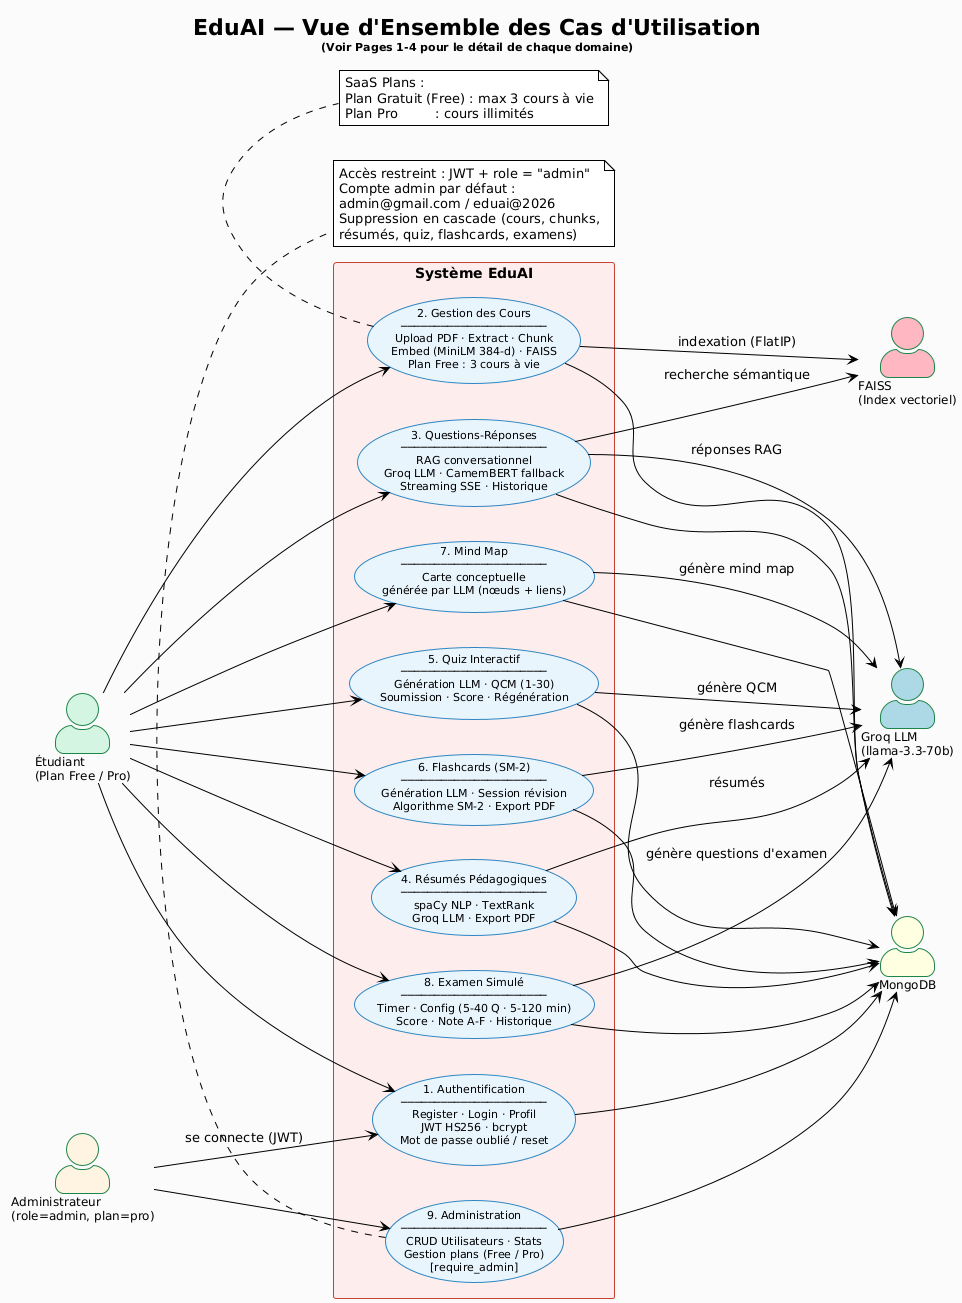
\includegraphics[width=\textwidth]{figures/uc_global.png}
\caption{Diagramme de cas d'utilisation global}
\end{figure}

\begin{figure}[H]
\centering
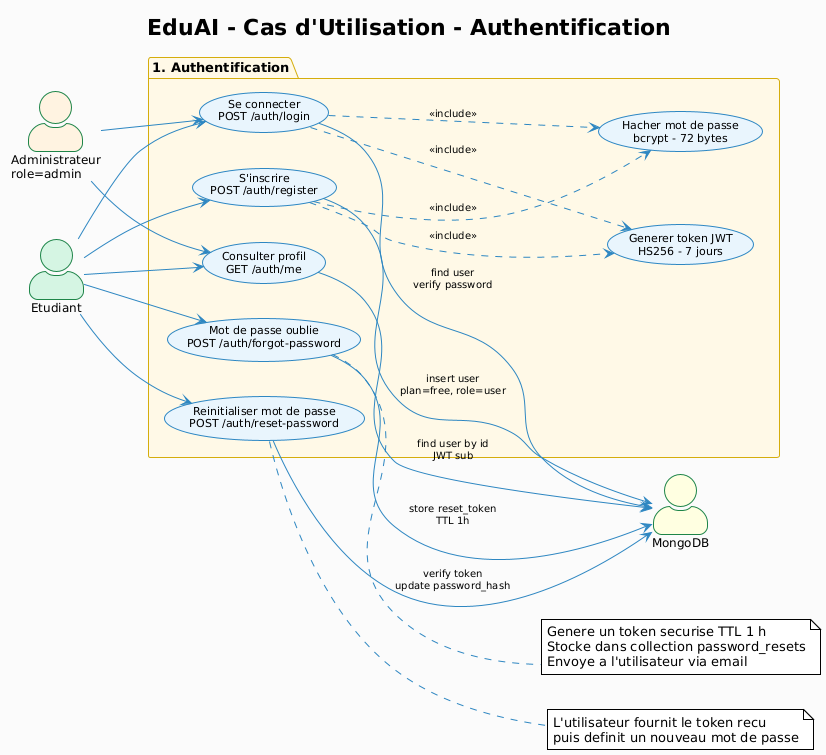
\includegraphics[width=0.85\textwidth]{figures/uc_p1_authentification.png}
\caption{Cas d'utilisation — P1 : Authentification}
\end{figure}

\begin{figure}[H]
\centering
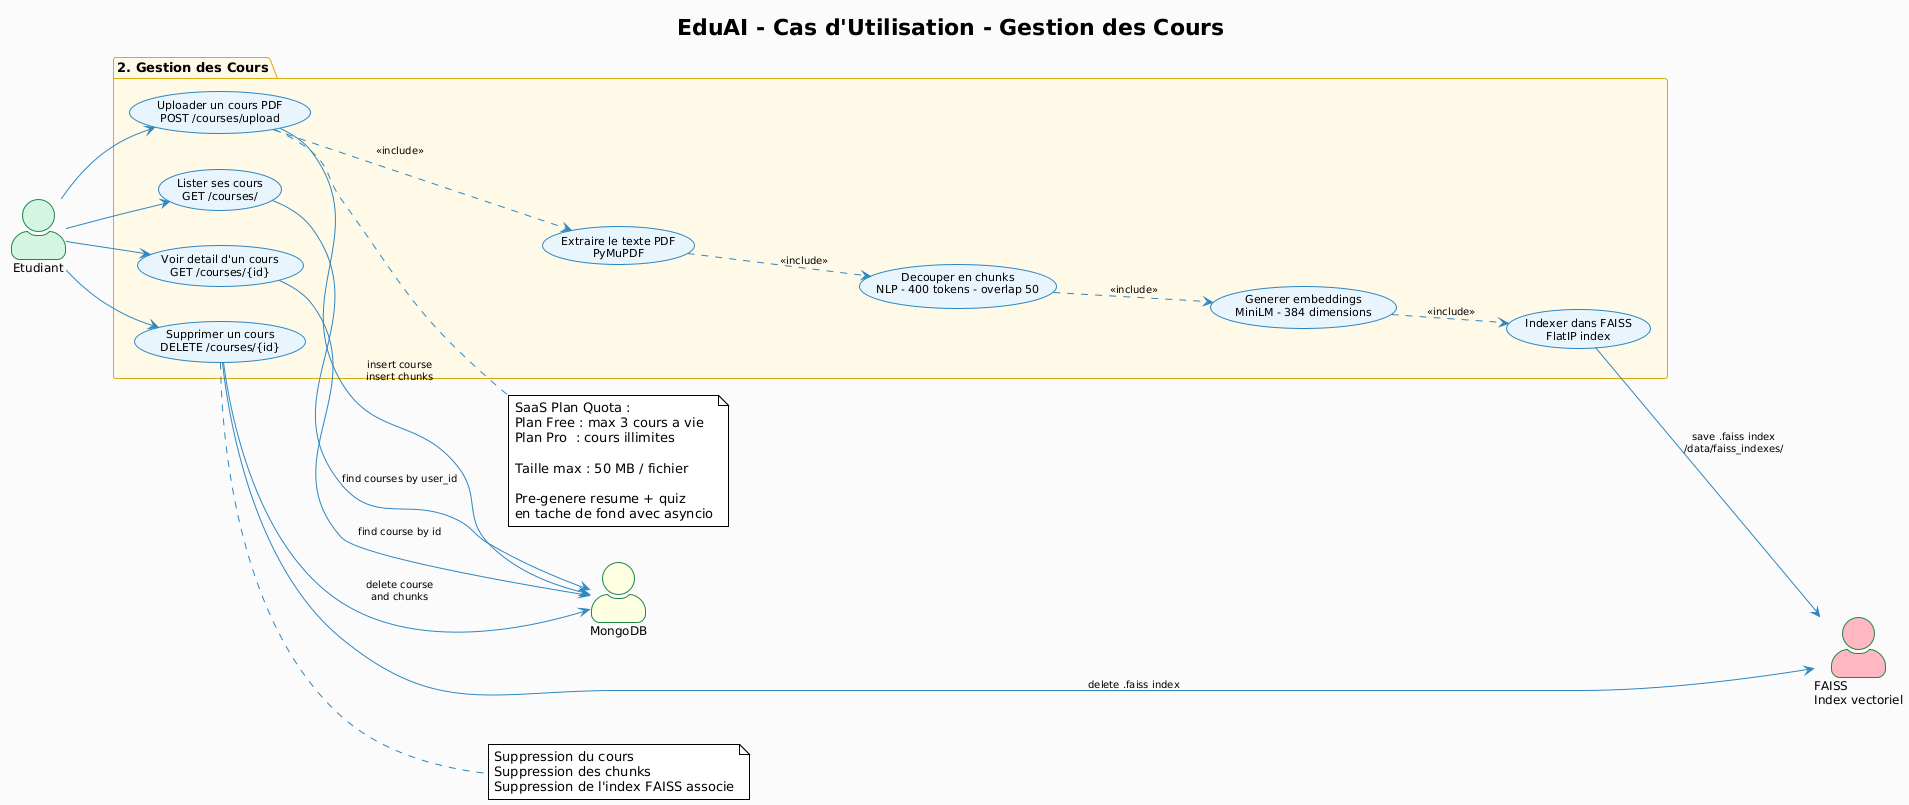
\includegraphics[width=0.85\textwidth]{figures/uc_p2_gestion_cours.png}
\caption{Cas d'utilisation — P2 : Gestion des cours}
\end{figure}

\begin{figure}[H]
\centering
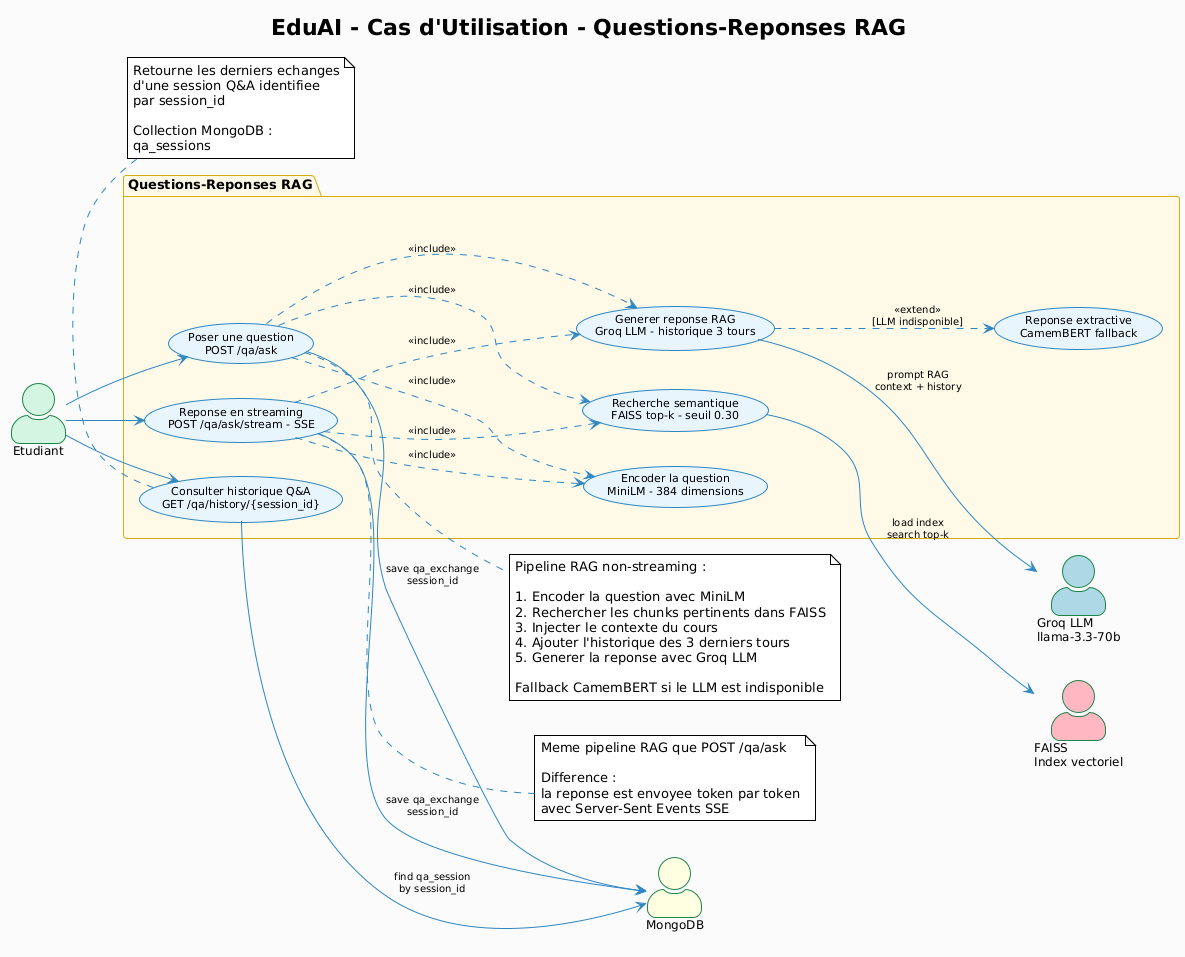
\includegraphics[width=0.85\textwidth]{figures/uc_p3_qa.png}
\caption{Cas d'utilisation — P3 : Questions-Réponses}
\end{figure}

\begin{figure}[H]
\centering
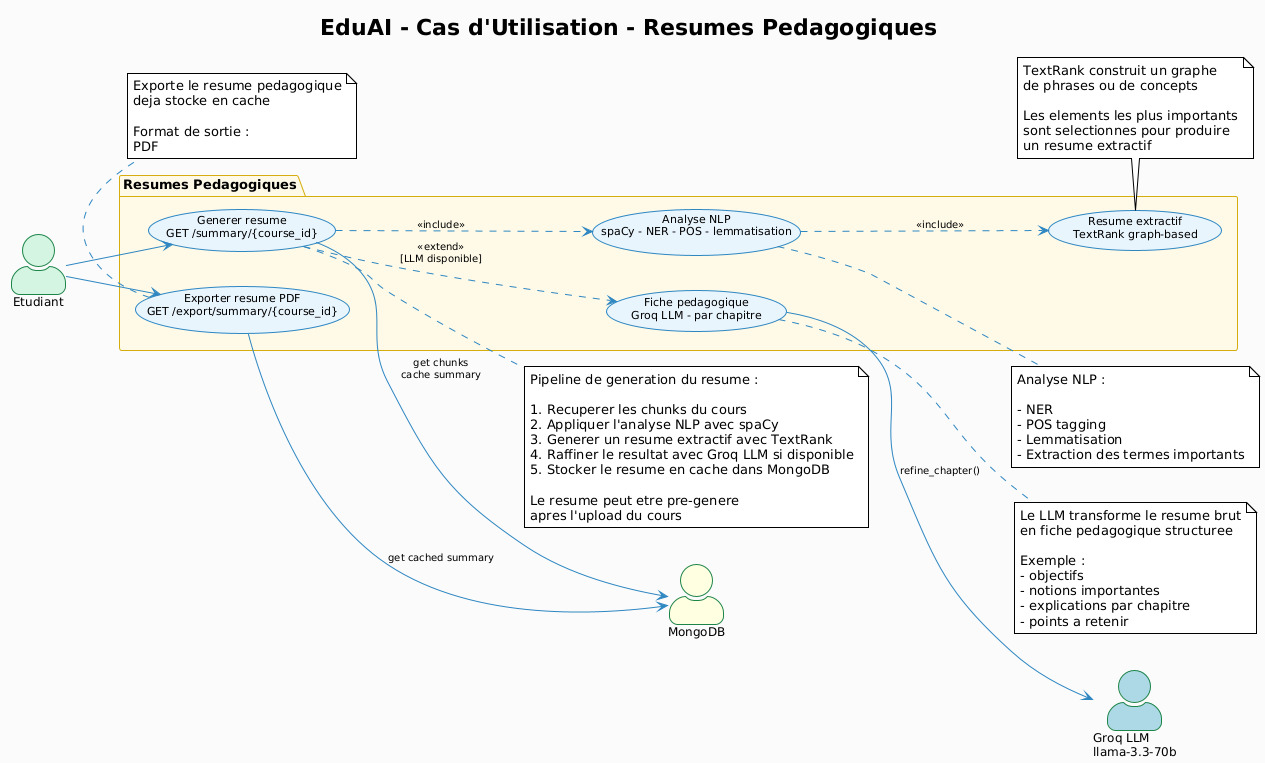
\includegraphics[width=0.85\textwidth]{figures/uc_p4_resumes.png}
\caption{Cas d'utilisation — P4 : Résumés}
\end{figure}

\begin{figure}[H]
\centering
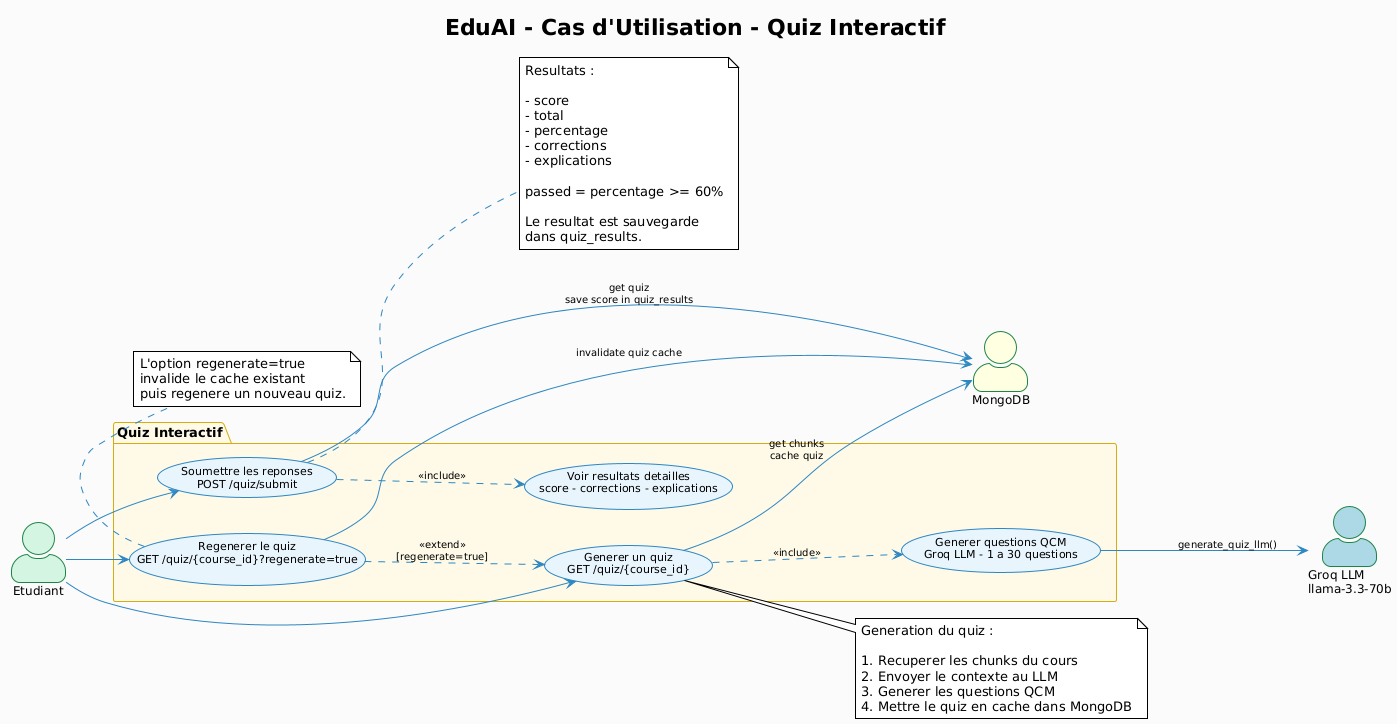
\includegraphics[width=0.85\textwidth]{figures/uc_p5_quiz.png}
\caption{Cas d'utilisation — P5 : Quiz}
\end{figure}

\begin{figure}[H]
\centering
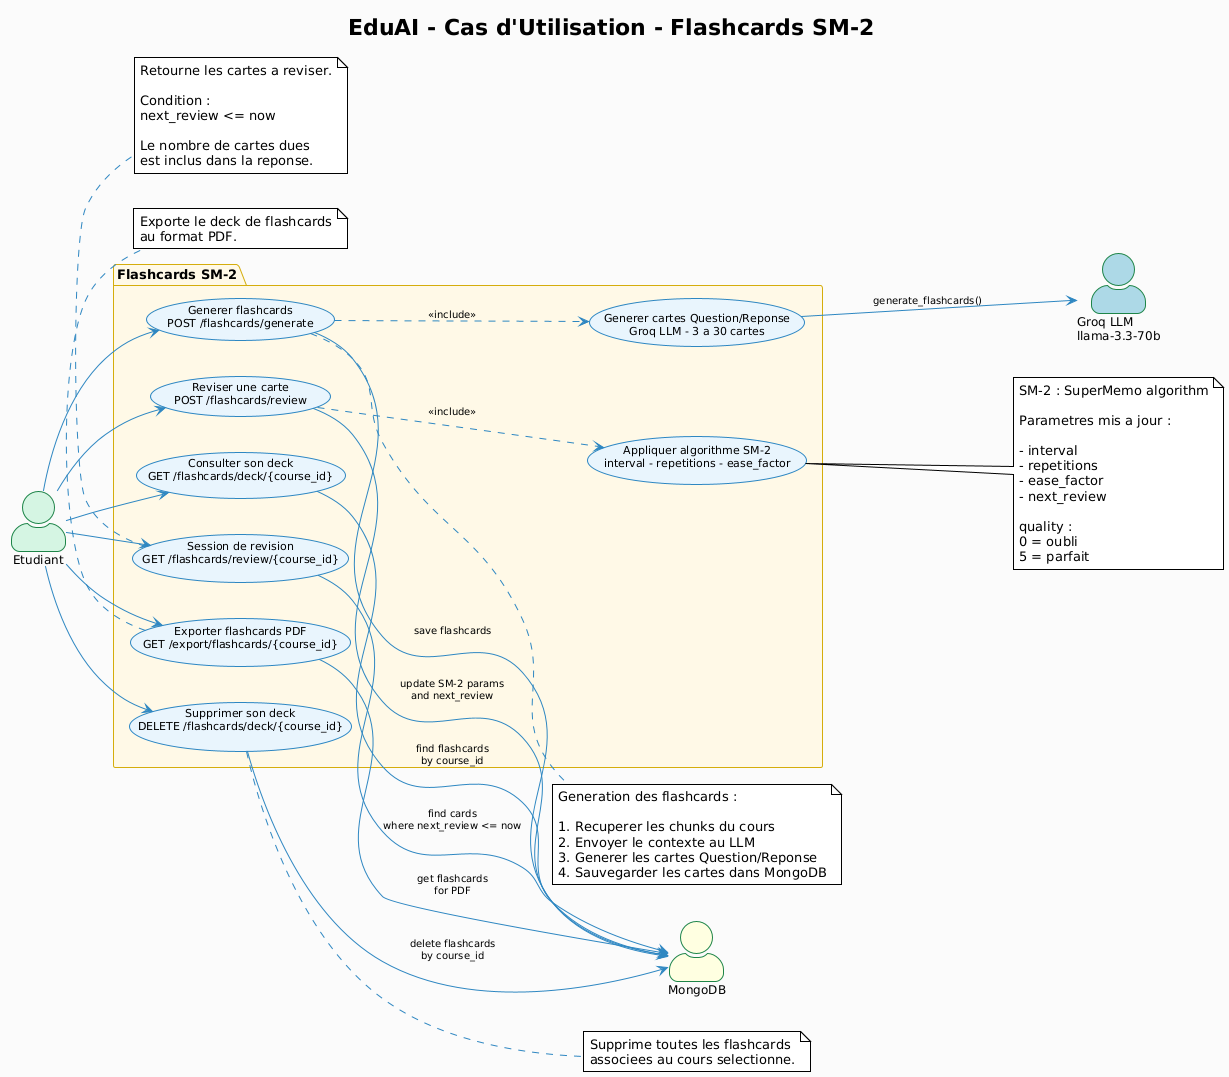
\includegraphics[width=0.85\textwidth]{figures/uc_p6_flashcards.png}
\caption{Cas d'utilisation — P6 : Flashcards}
\end{figure}

\begin{figure}[H]
\centering
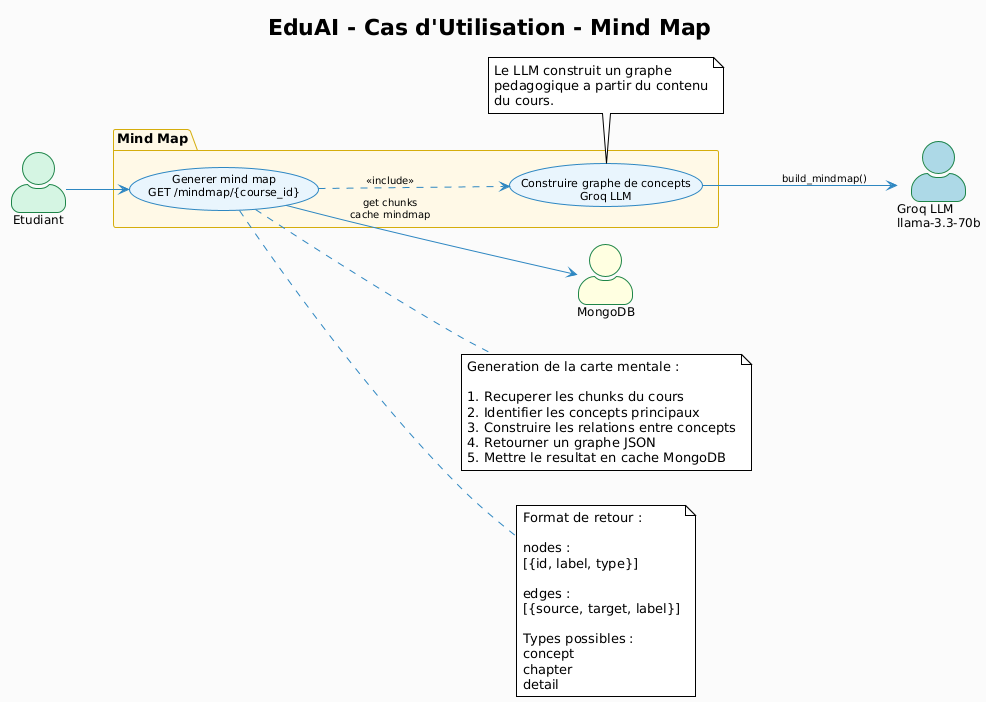
\includegraphics[width=0.85\textwidth]{figures/uc_p7_mindmap.png}
\caption{Cas d'utilisation — P7 : Carte mentale}
\end{figure}

\begin{figure}[H]
\centering
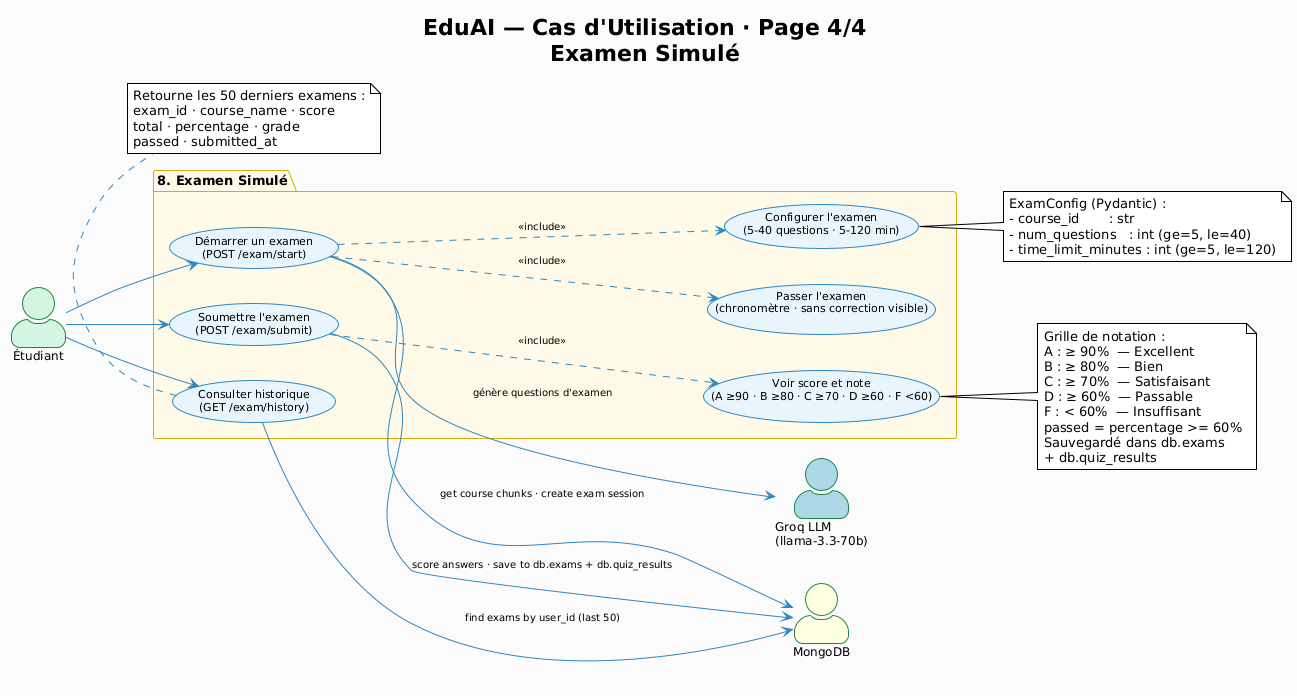
\includegraphics[width=0.85\textwidth]{figures/uc_p8_examen.png}
\caption{Cas d'utilisation — P8 : Examen}
\end{figure}

\begin{figure}[H]
\centering
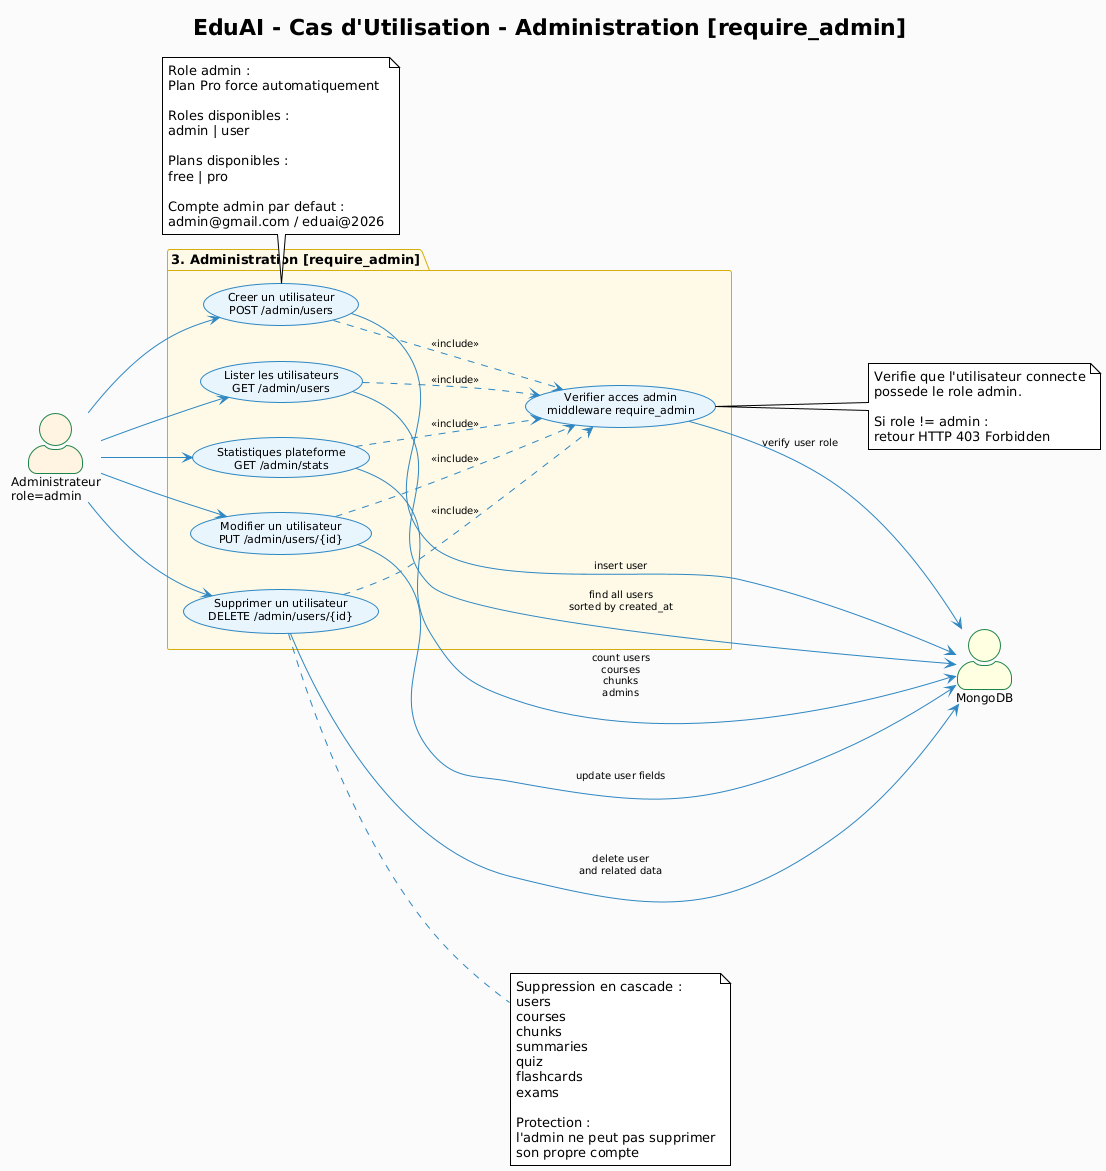
\includegraphics[width=0.85\textwidth]{figures/uc_p9_administration.png}
\caption{Cas d'utilisation — P9 : Administration}
\end{figure}

% ── Annexe B : Diagrammes de séquence ─────────────────────────────────────
\chapter{Diagrammes de séquence}

\begin{figure}[H]
\centering
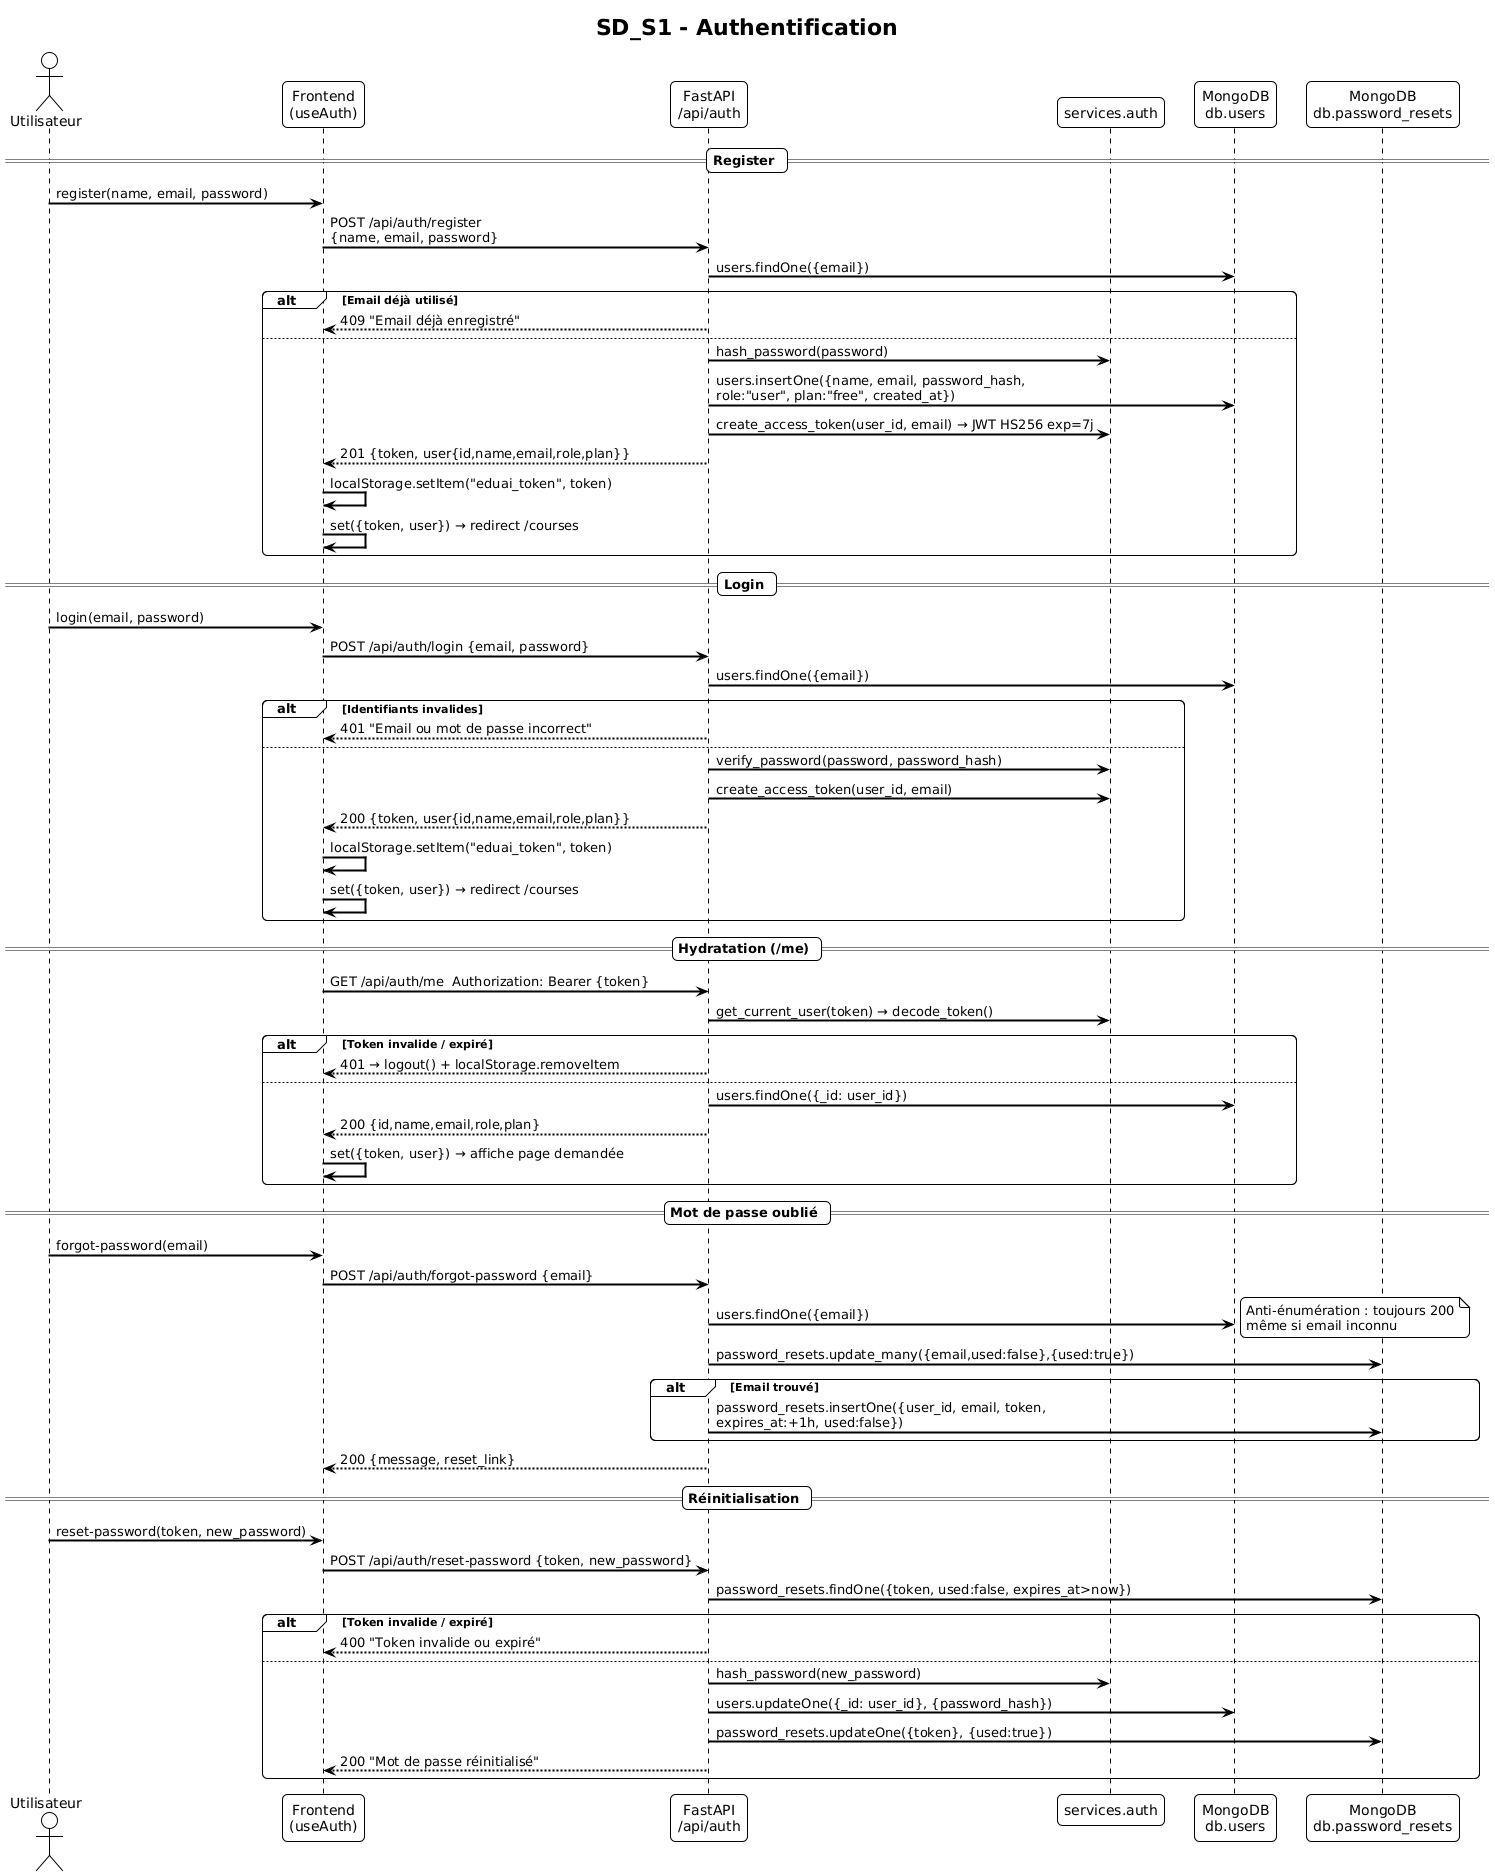
\includegraphics[width=\textwidth]{figures/sd_s1_auth.png}
\caption{Diagramme de séquence — Authentification}
\end{figure}

\begin{figure}[H]
\centering
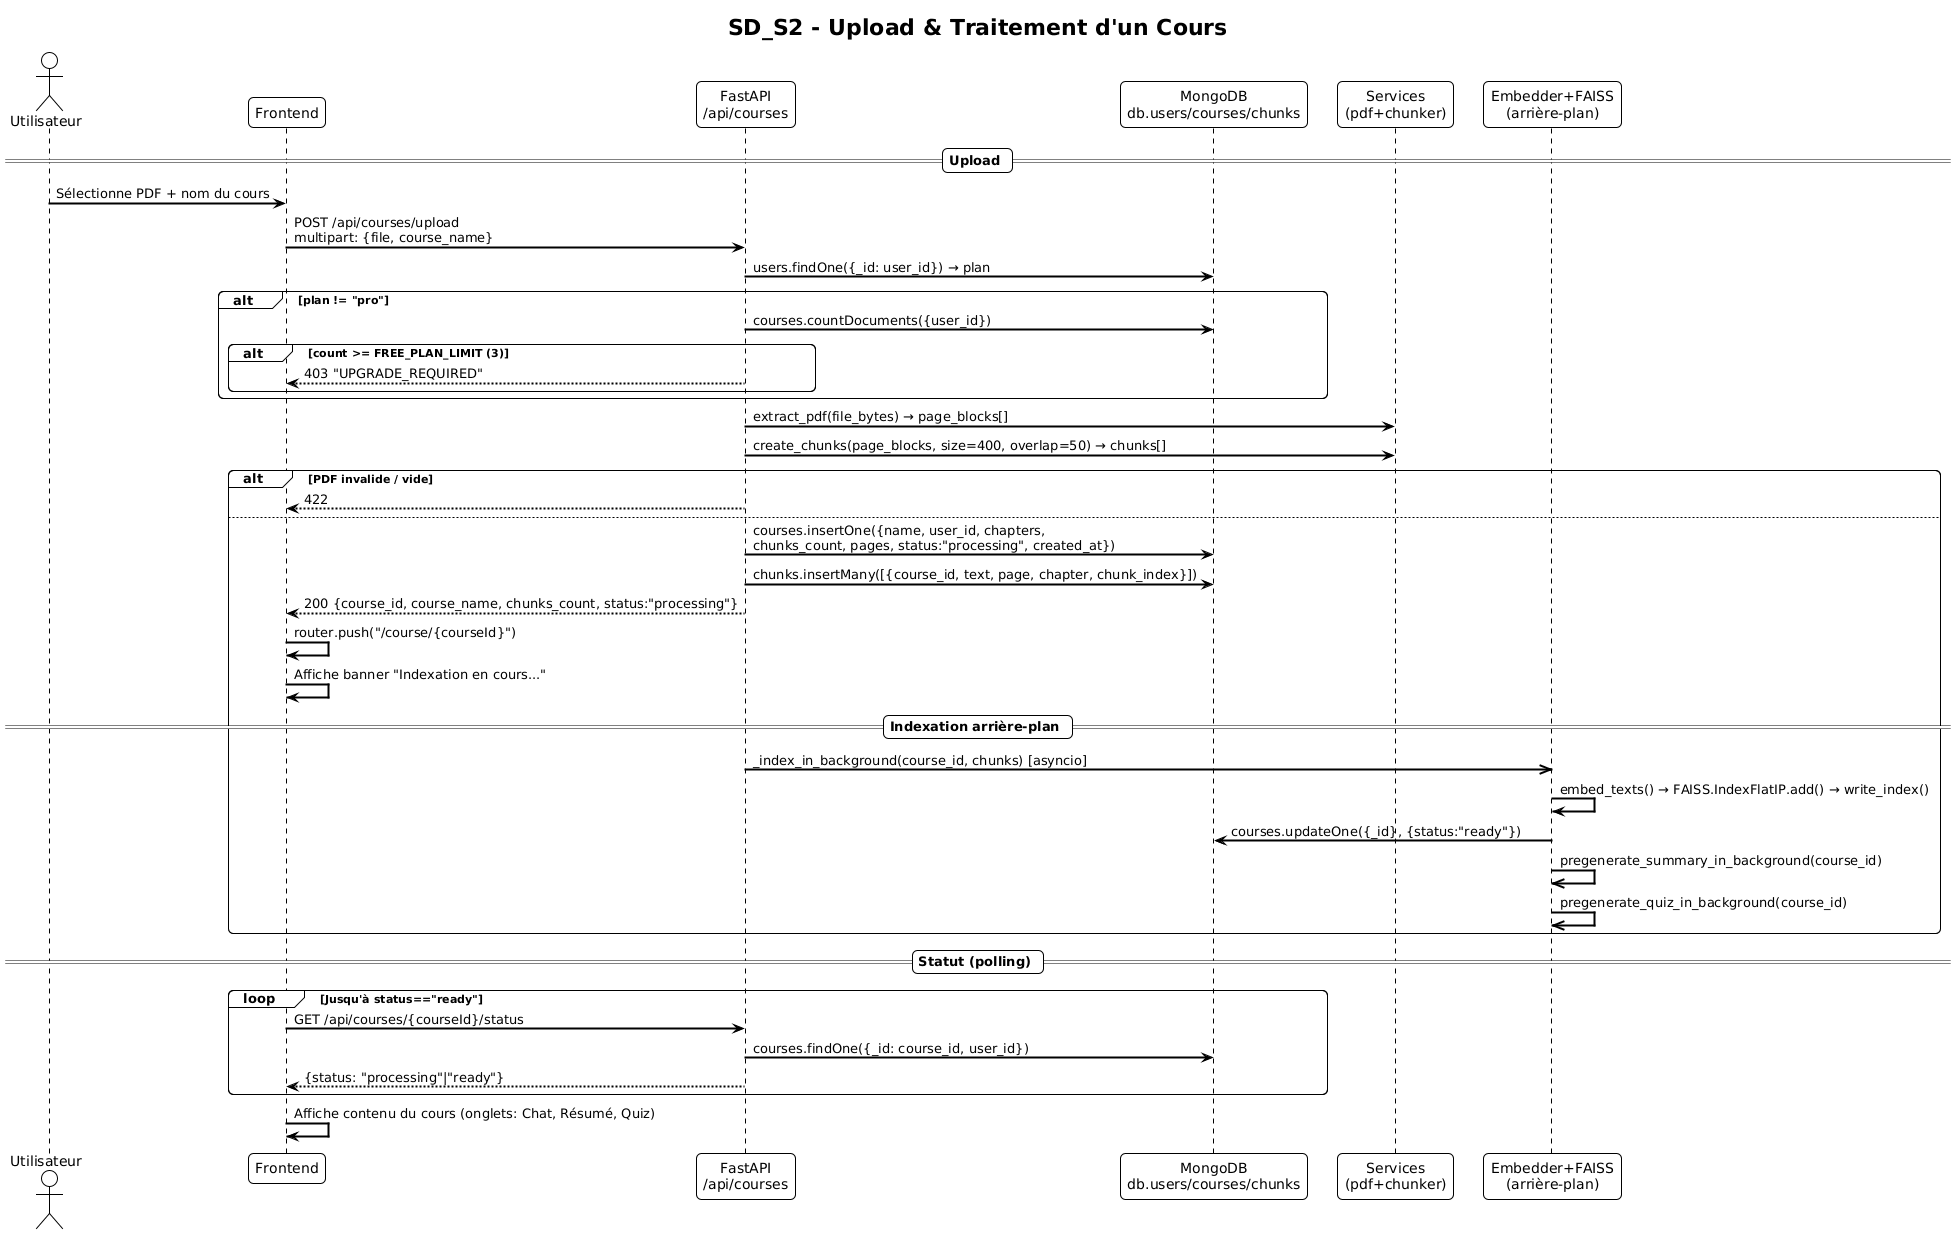
\includegraphics[width=\textwidth]{figures/sd_s2_upload.png}
\caption{Diagramme de séquence — Upload de cours}
\end{figure}

\begin{figure}[H]
\centering
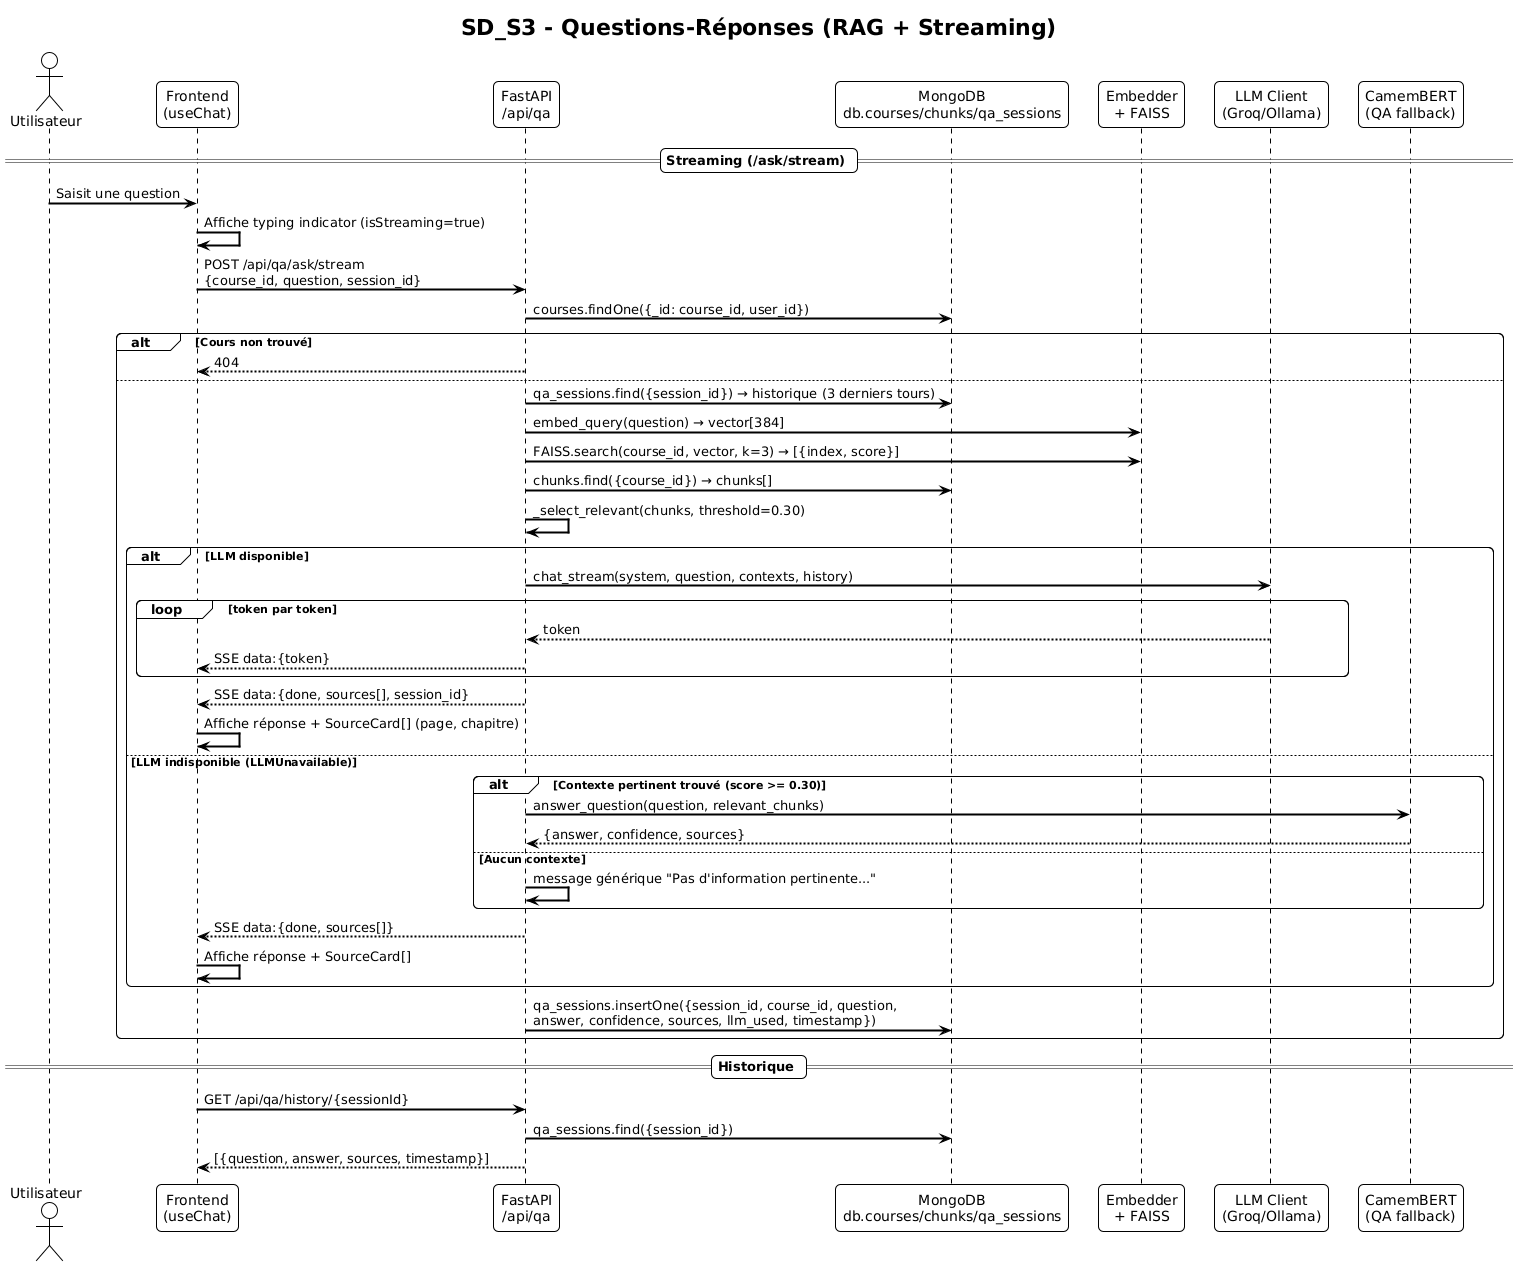
\includegraphics[width=\textwidth]{figures/sd_s3_qa.png}
\caption{Diagramme de séquence — Questions-Réponses (RAG)}
\end{figure}

\begin{figure}[H]
\centering
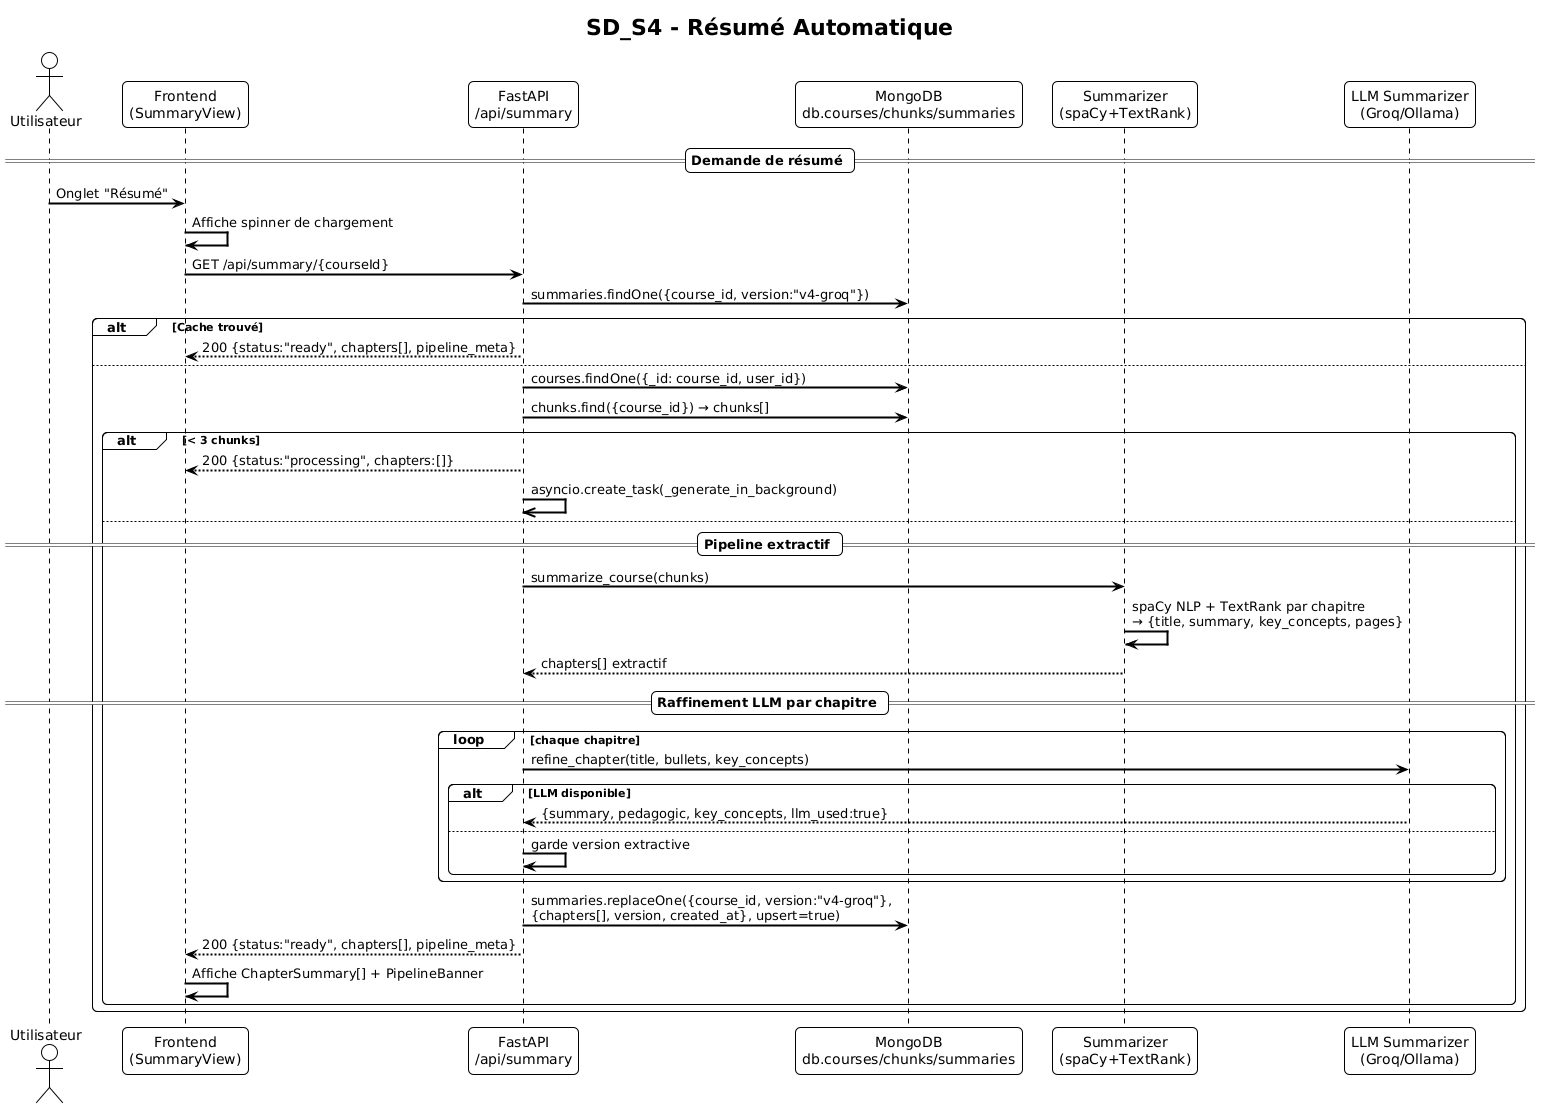
\includegraphics[width=\textwidth]{figures/sd_s4_summary.png}
\caption{Diagramme de séquence — Génération de résumé}
\end{figure}

\begin{figure}[H]
\centering
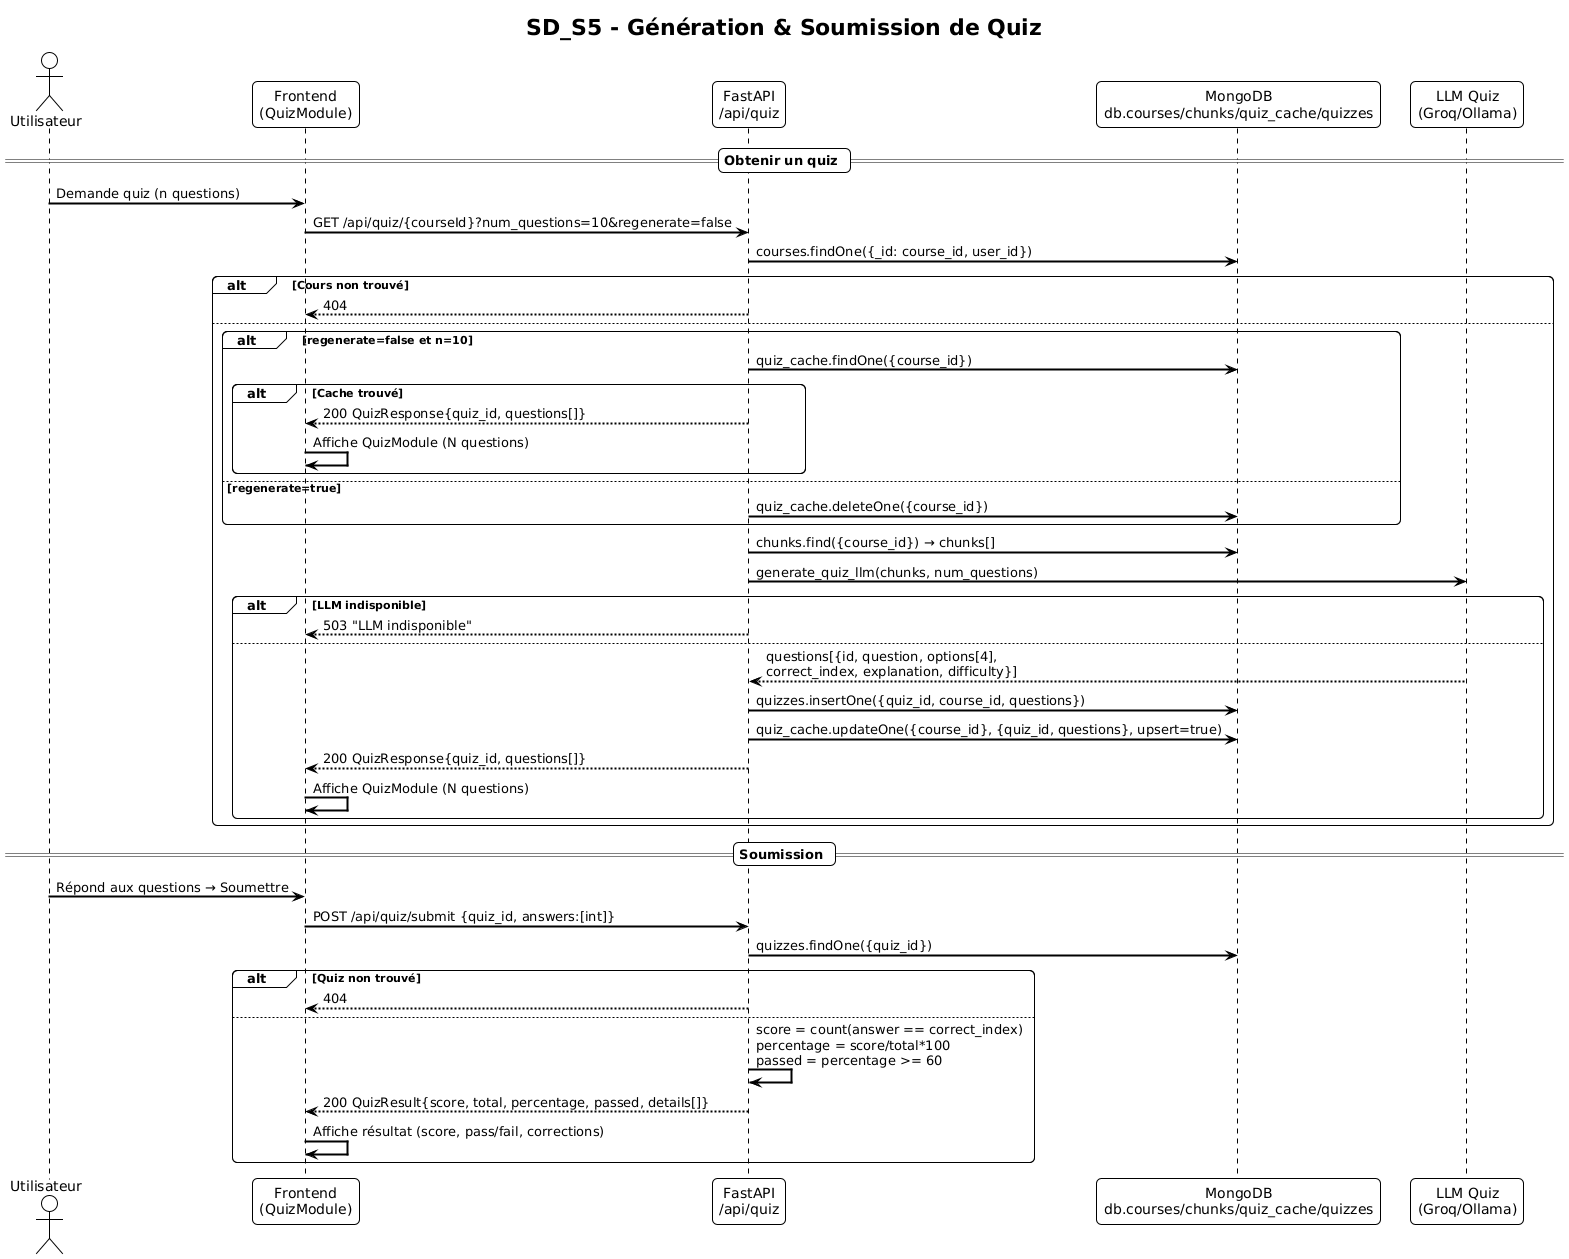
\includegraphics[width=\textwidth]{figures/sd_s5_quiz.png}
\caption{Diagramme de séquence — Quiz}
\end{figure}

\begin{figure}[H]
\centering
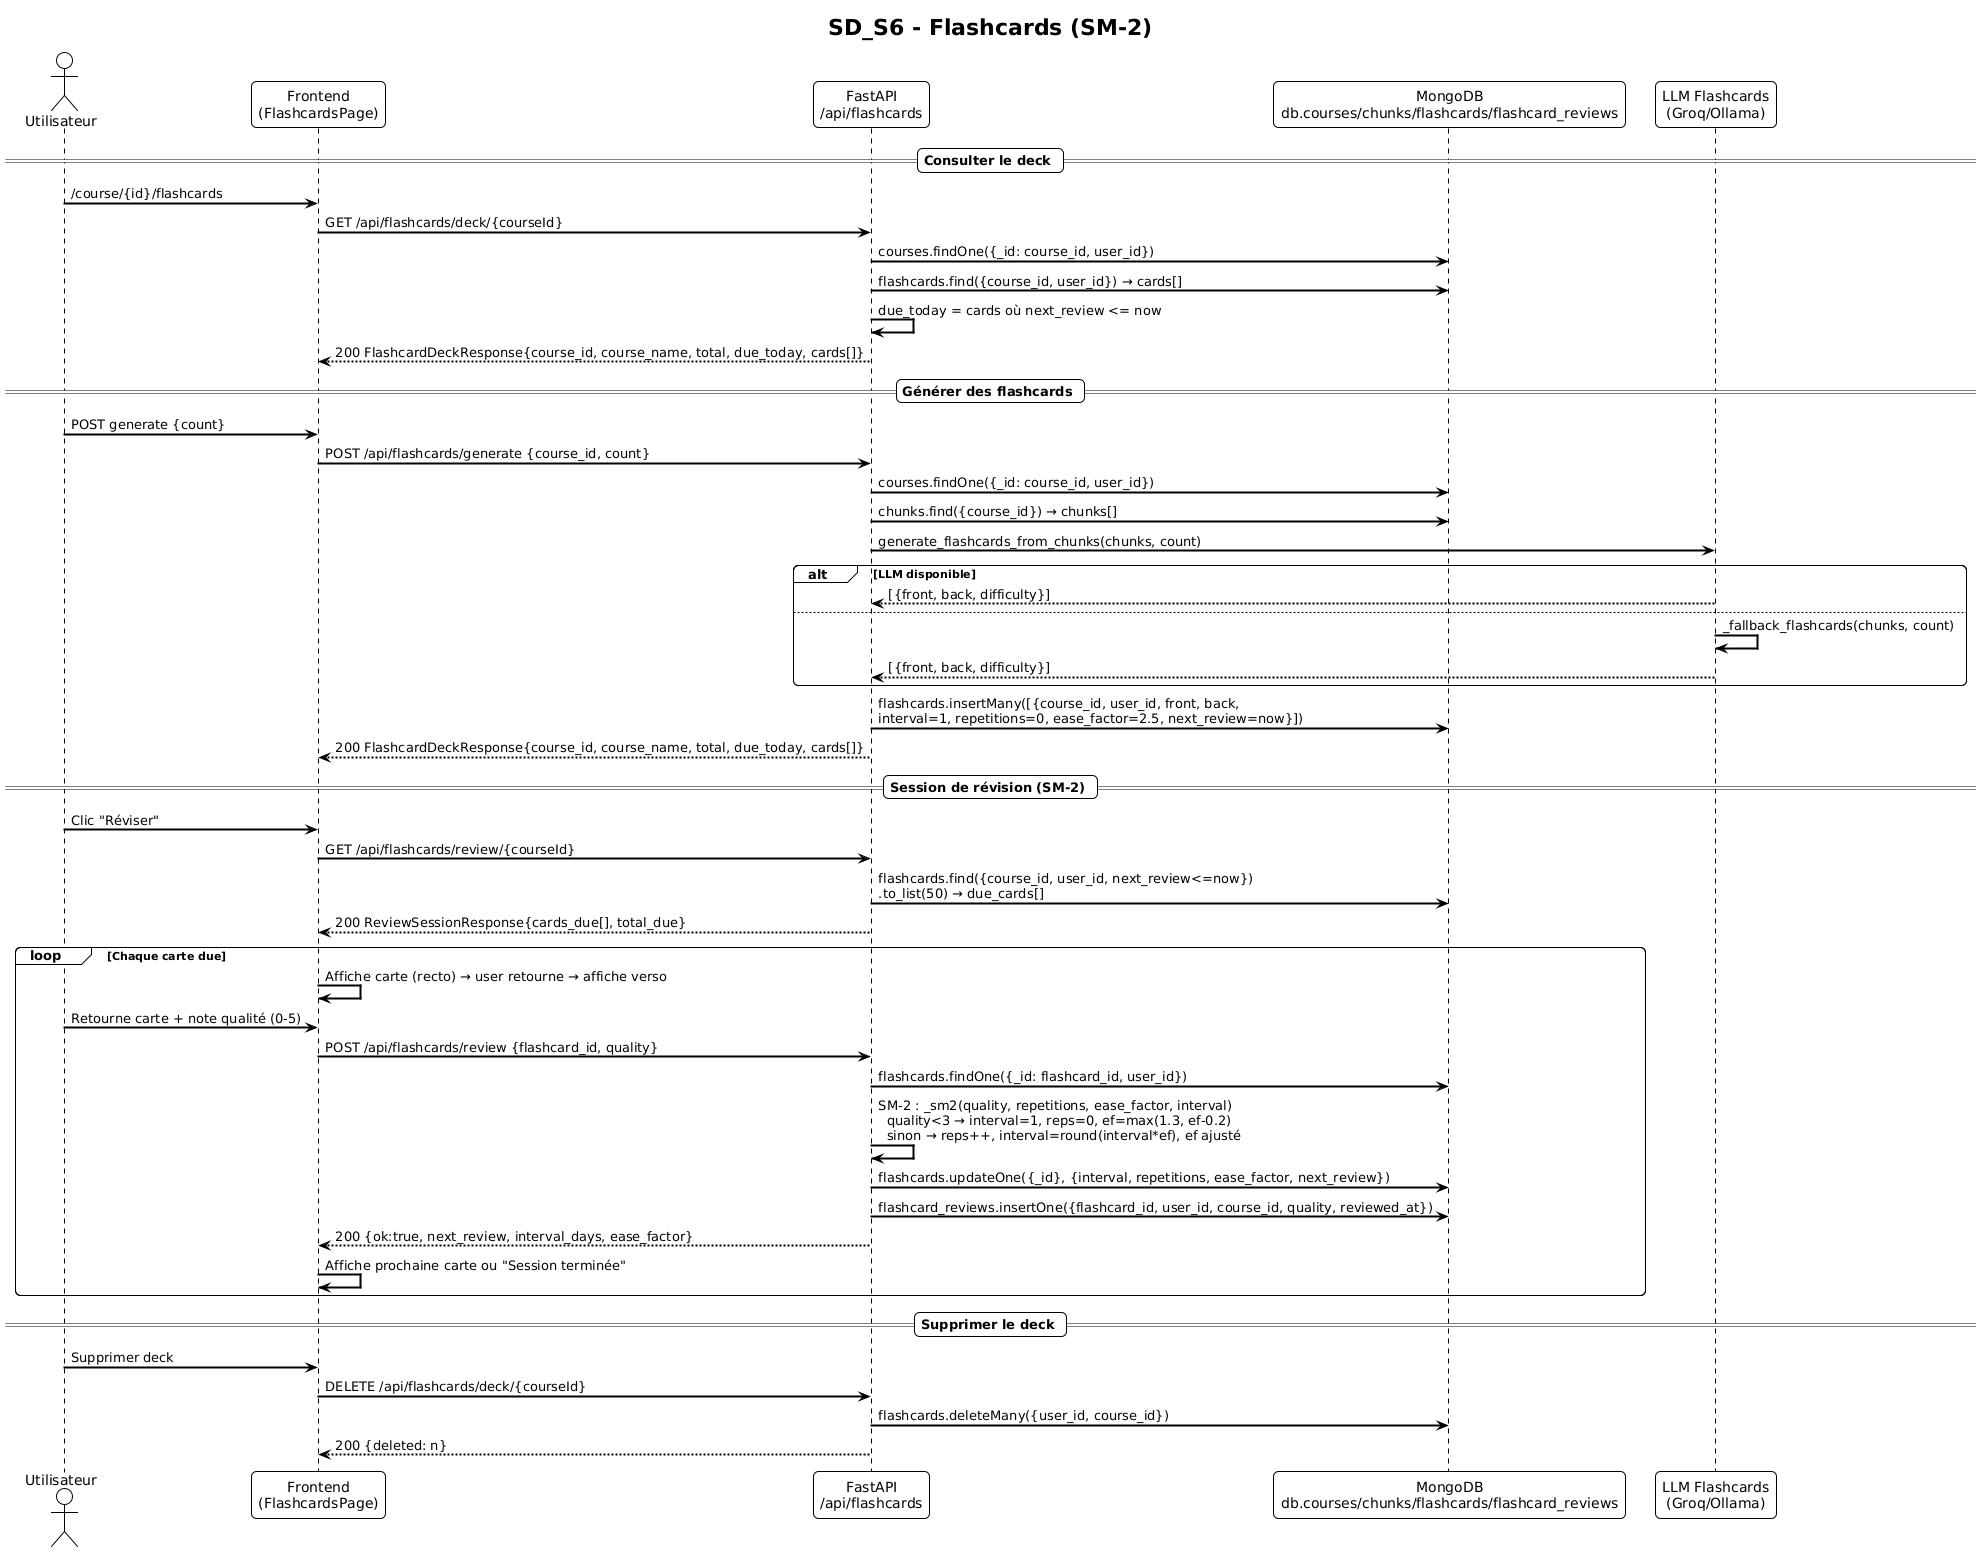
\includegraphics[width=\textwidth]{figures/sd_s6_flashcards.png}
\caption{Diagramme de séquence — Flashcards}
\end{figure}

\begin{figure}[H]
\centering
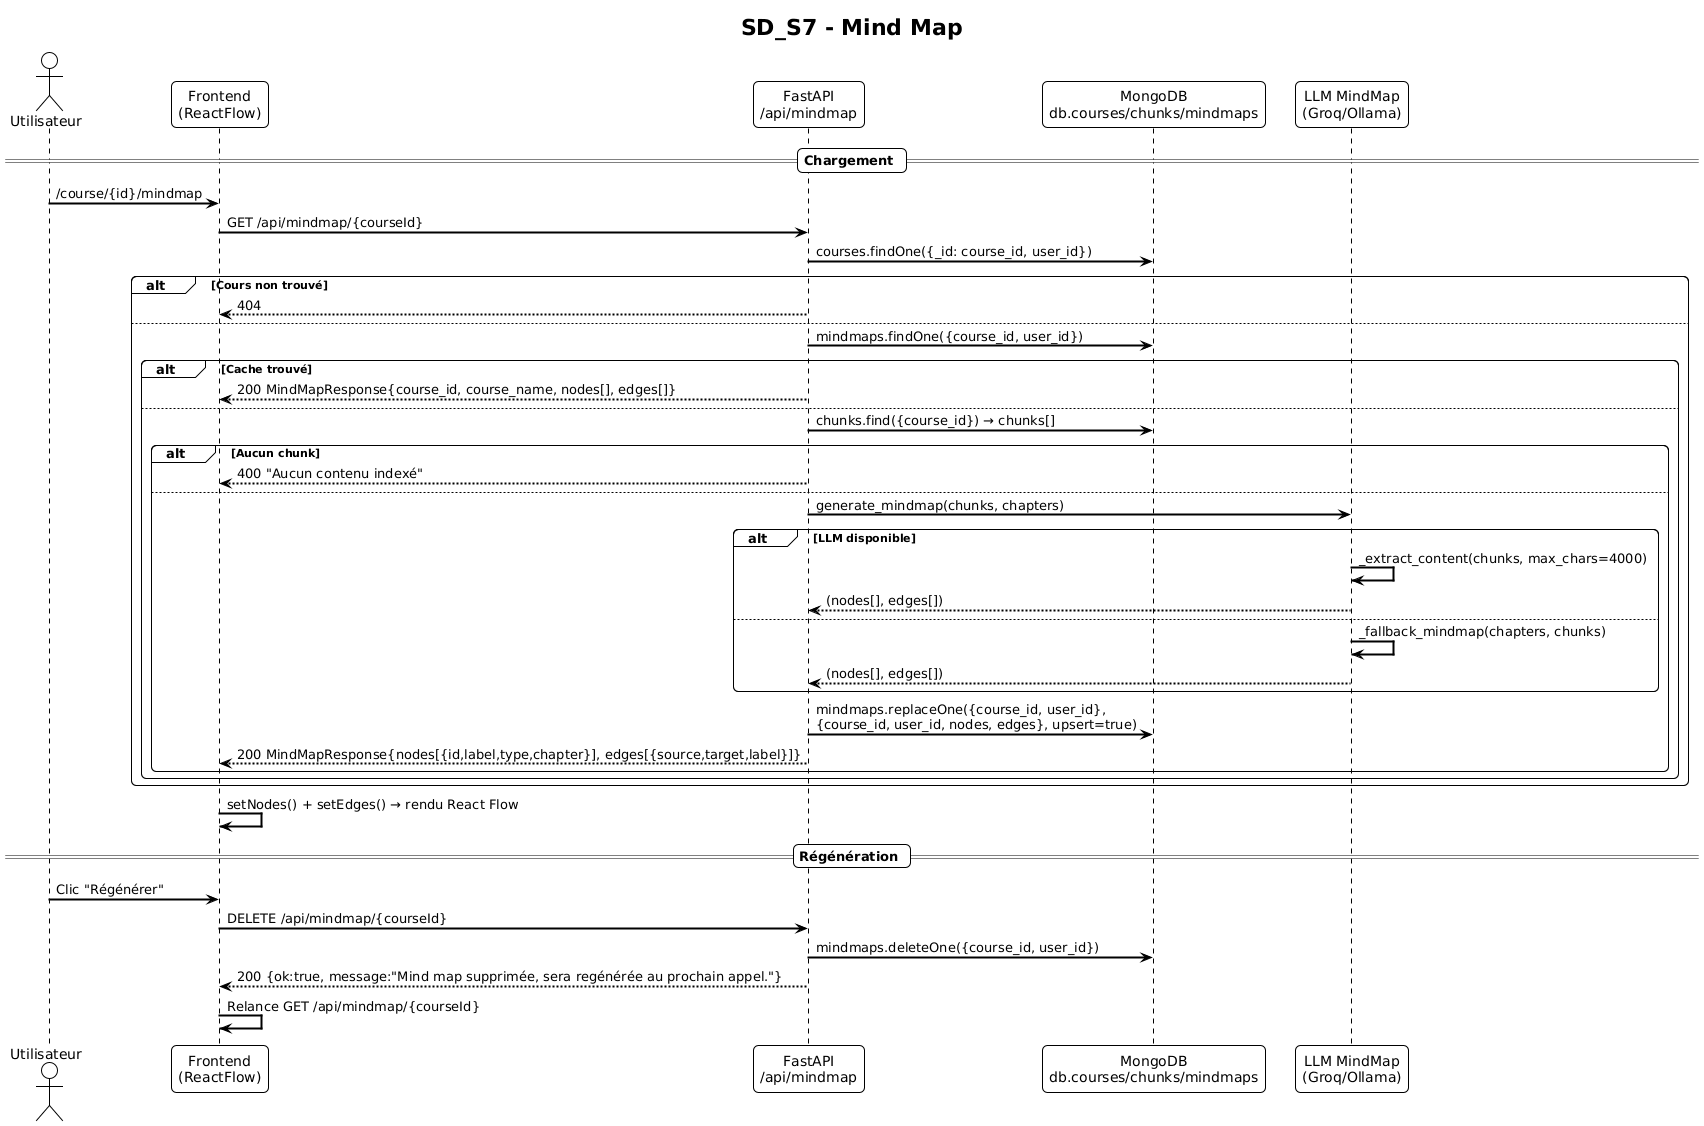
\includegraphics[width=\textwidth]{figures/sd_s7_mindmap.png}
\caption{Diagramme de séquence — Carte mentale}
\end{figure}

\begin{figure}[H]
\centering
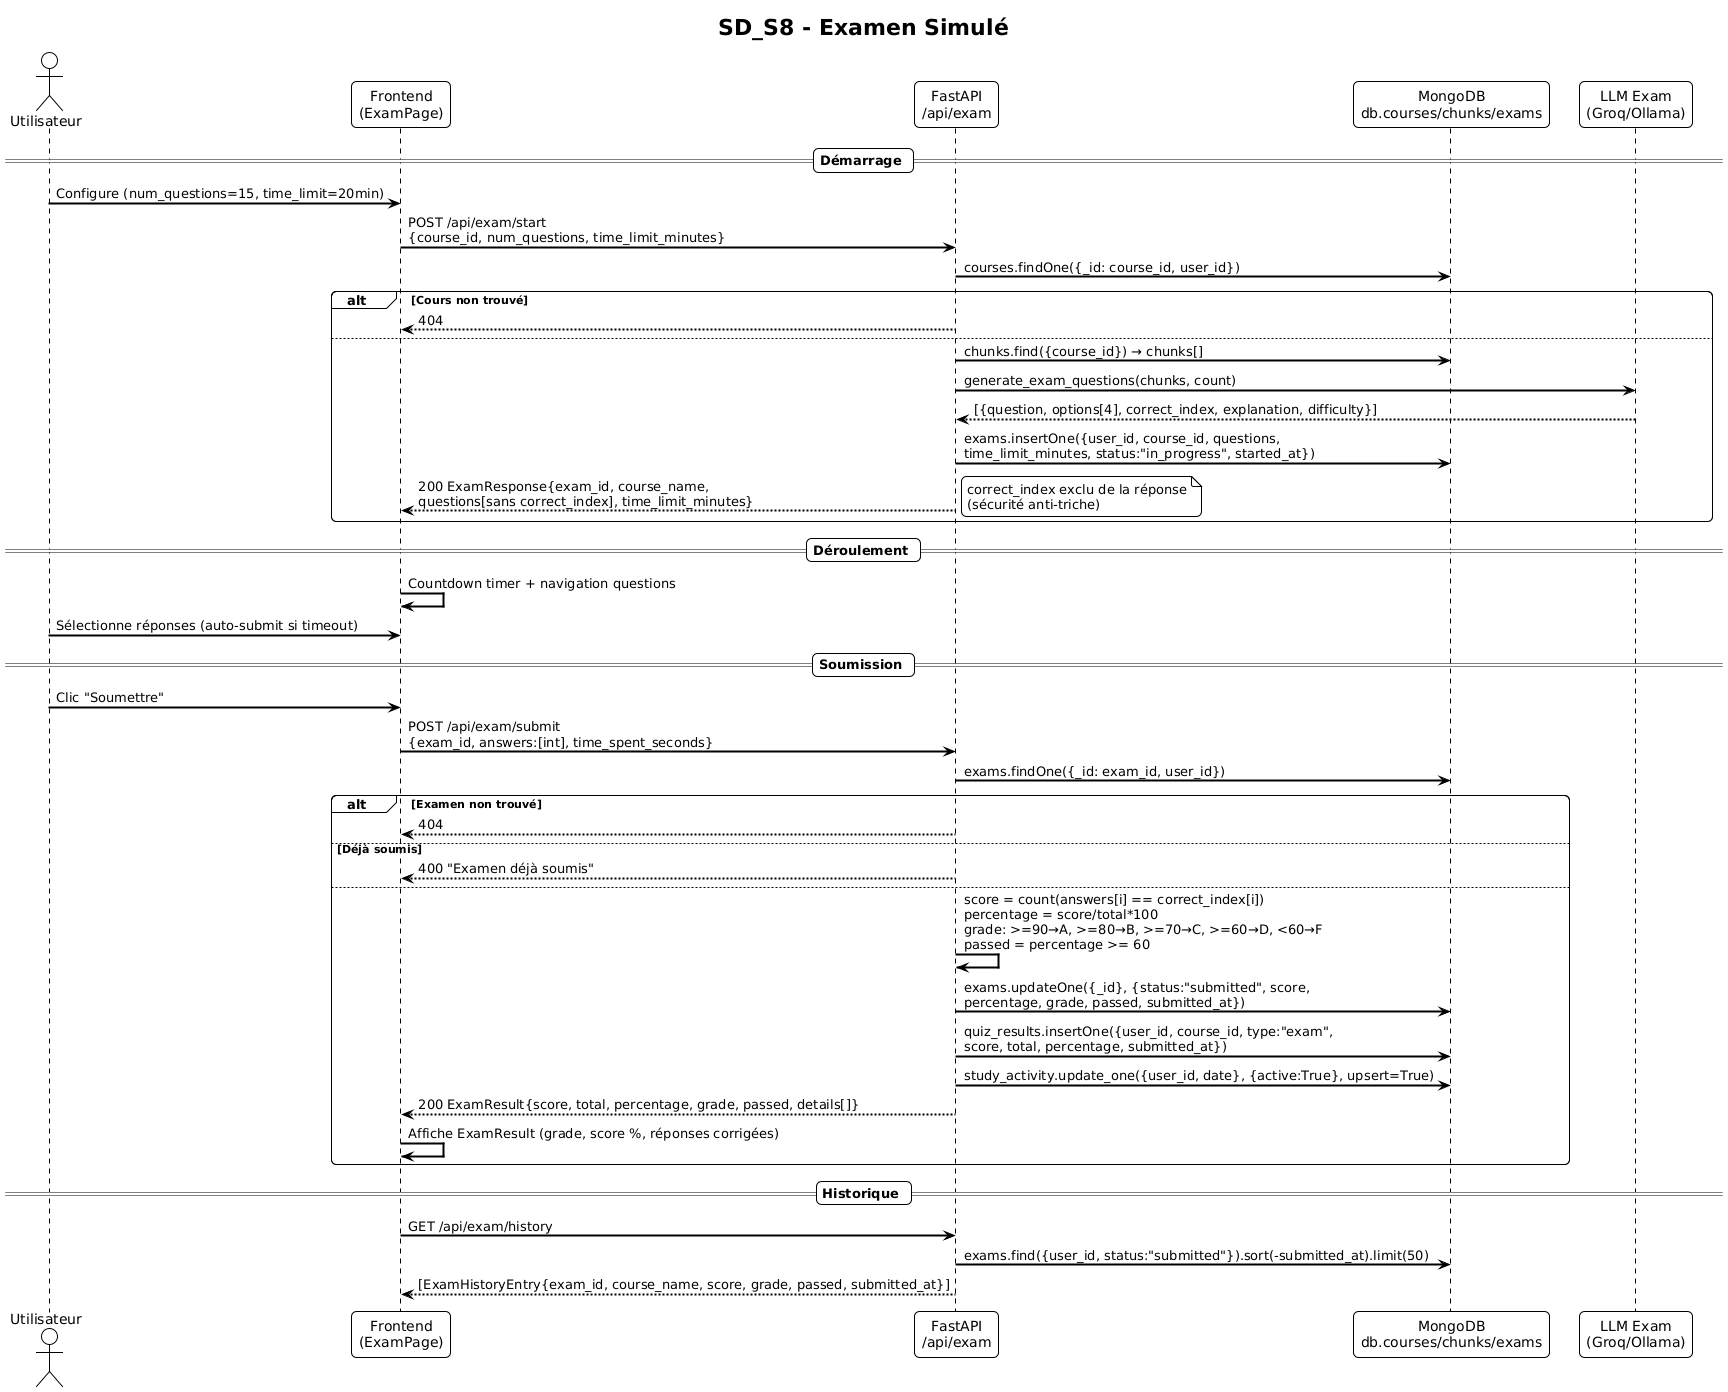
\includegraphics[width=\textwidth]{figures/sd_s8_exam.png}
\caption{Diagramme de séquence — Examen}
\end{figure}

\begin{figure}[H]
\centering
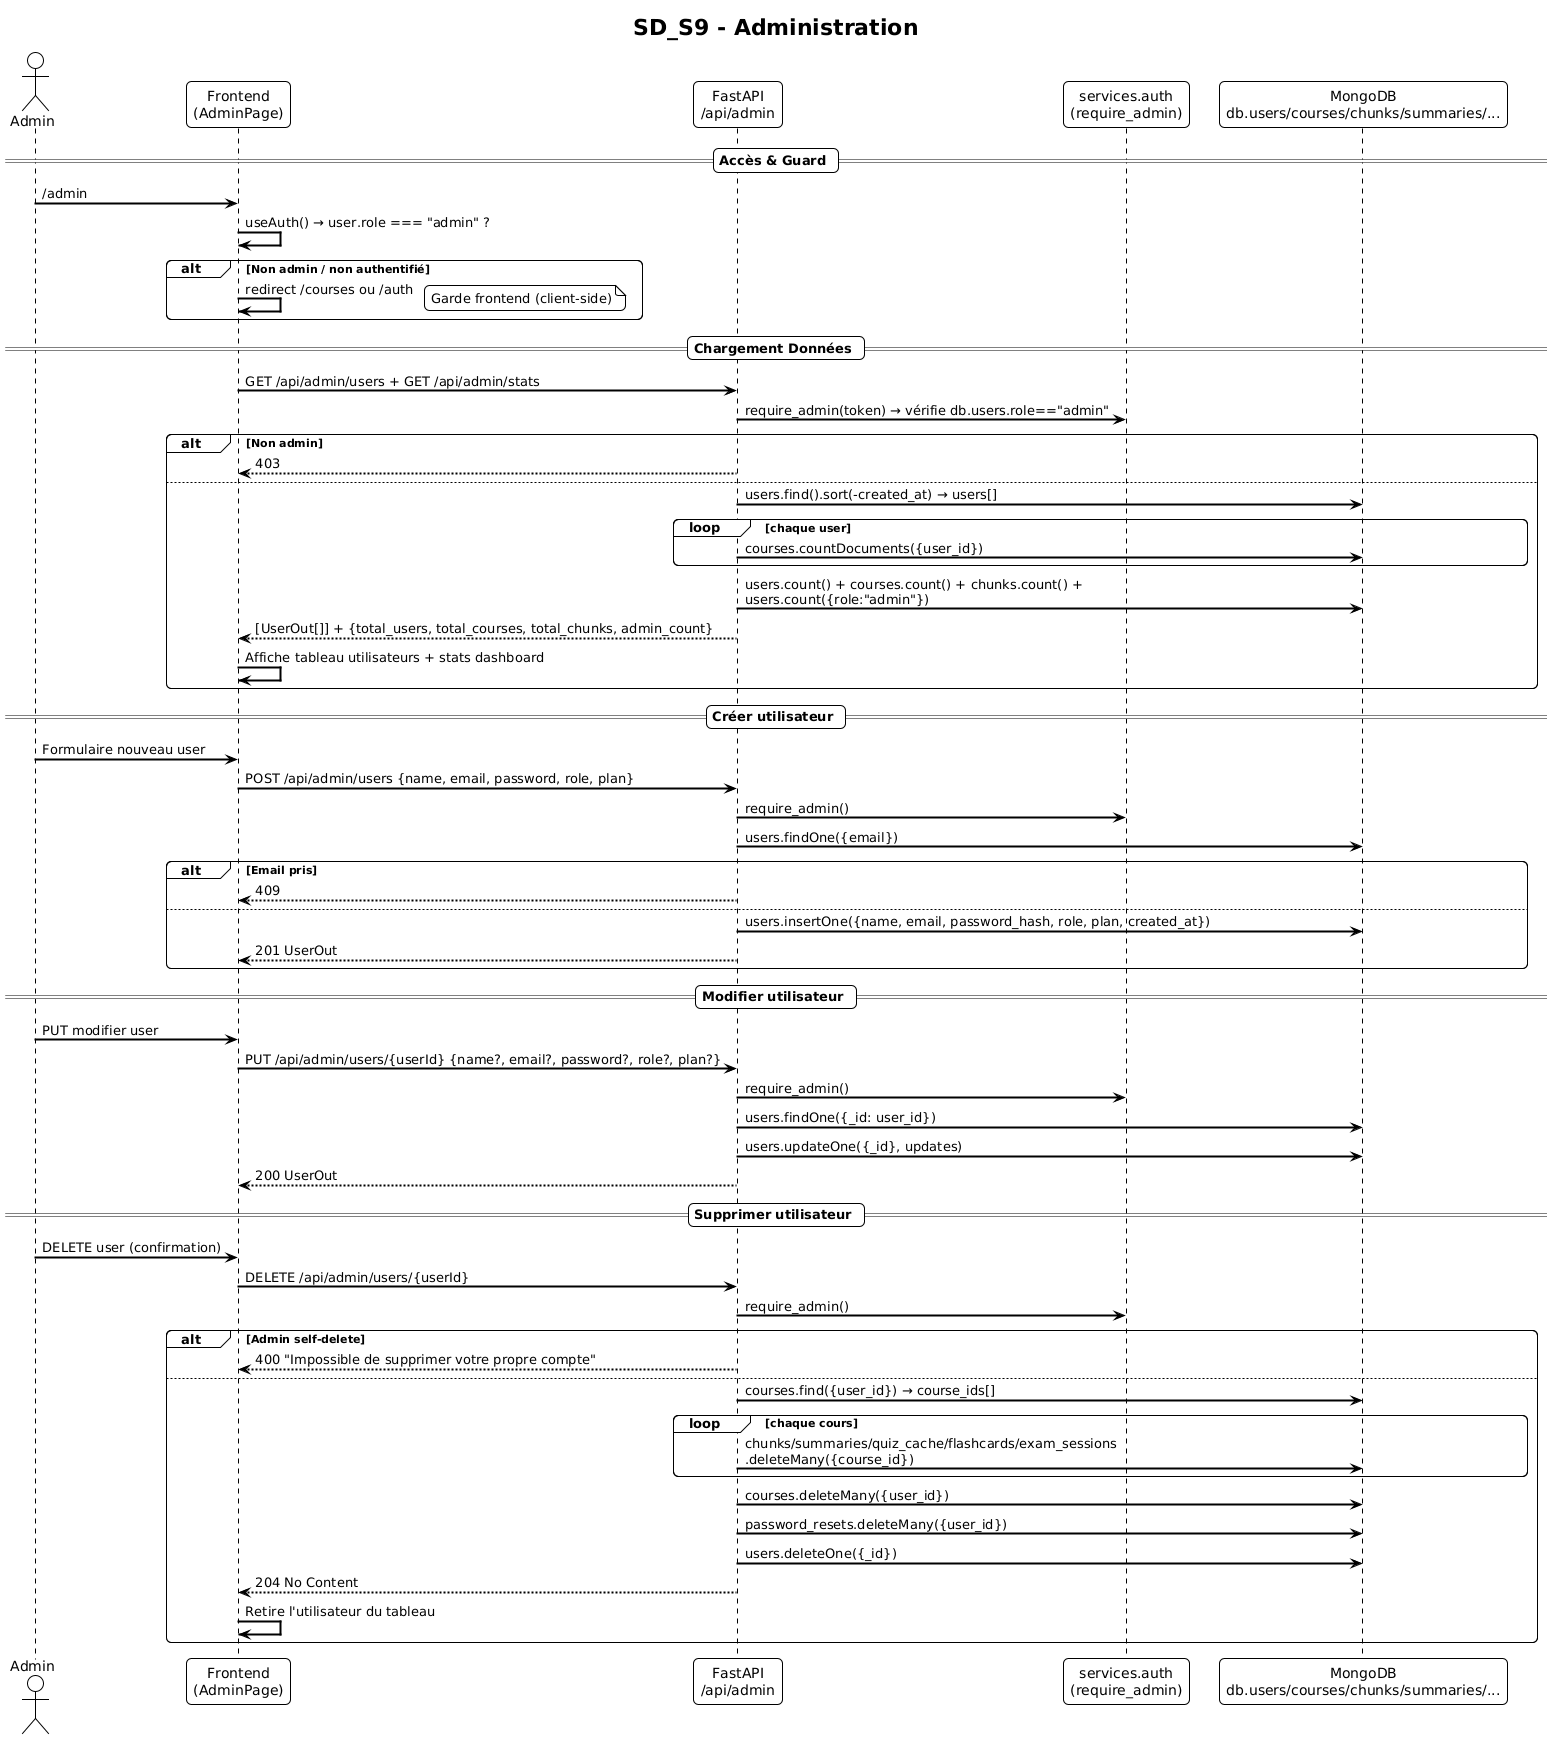
\includegraphics[width=\textwidth]{figures/sd_s9_admin.png}
\caption{Diagramme de séquence — Administration}
\end{figure}

% ── Annexe C : Modèle Logique de Données ──────────────────────────────────
\chapter{Modèle Logique de Données}

\begin{figure}[H]
\centering
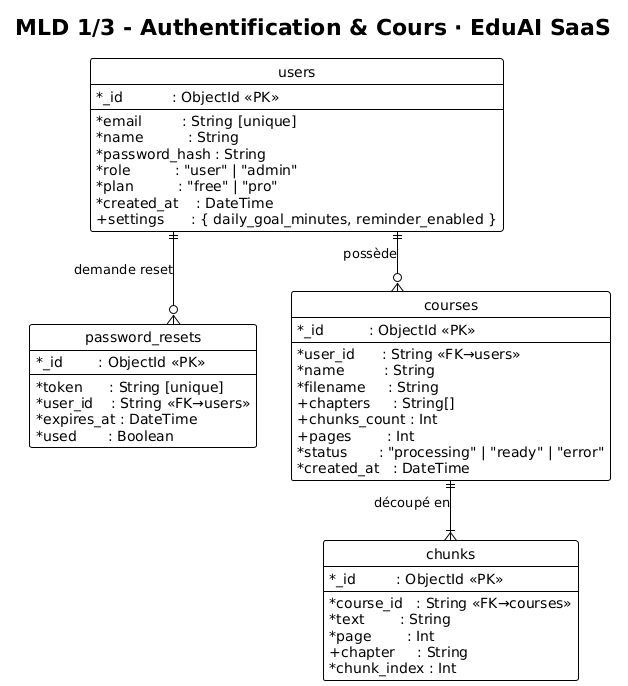
\includegraphics[width=\textwidth]{figures/mld_1_auth_cours.png}
\caption{MLD 1/3 — Authentification et Cours (4 collections)}
\end{figure}

\begin{figure}[H]
\centering
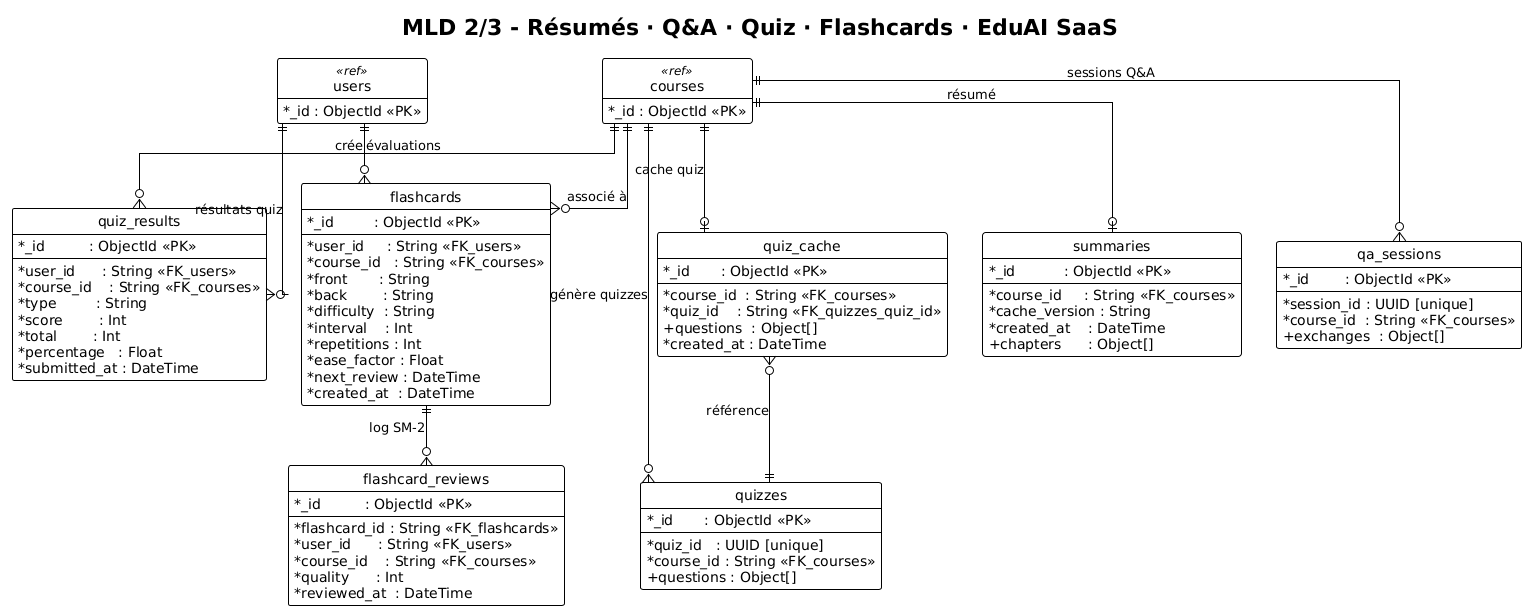
\includegraphics[width=\textwidth]{figures/mld_2_quiz_flash.png}
\caption{MLD 2/3 — Résumés, Q\&A, Quiz et Flashcards (7 collections)}
\end{figure}

\begin{figure}[H]
\centering
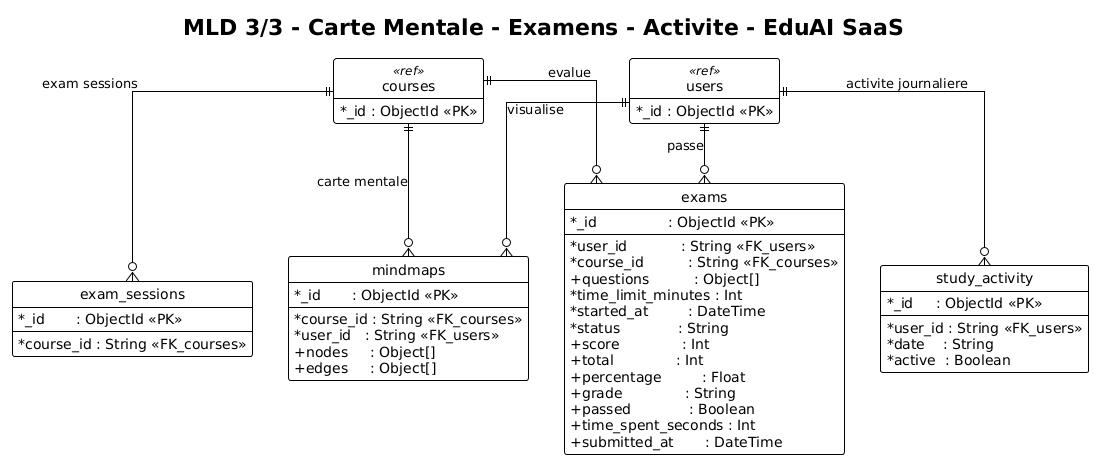
\includegraphics[width=\textwidth]{figures/mld_3_exam_activite.png}
\caption{MLD 3/3 — Carte mentale, Examens et Activité (4 collections)}
\end{figure}

% ── Annexe D : Interfaces utilisateur ─────────────────────────────────────
\chapter{Interfaces utilisateur}

\begin{figure}[H]
\centering
\fbox{\parbox{0.9\textwidth}{\centering\vspace{4cm}
\textit{[Capture d'écran : Page d'accueil — Hero section avec CTA]}
\vspace{4cm}}}
\caption{Page d'accueil EduAI}
\end{figure}

\begin{figure}[H]
\centering
\fbox{\parbox{0.9\textwidth}{\centering\vspace{3.5cm}
\textit{[Capture d'écran : Formulaire d'inscription / connexion]}
\vspace{3.5cm}}}
\caption{Interface d'authentification}
\end{figure}

\begin{figure}[H]
\centering
\fbox{\parbox{0.9\textwidth}{\centering\vspace{4cm}
\textit{[Capture d'écran : Dashboard avec les cartes des cours]}
\vspace{4cm}}}
\caption{Tableau de bord — Mes cours}
\end{figure}

\begin{figure}[H]
\centering
\fbox{\parbox{0.9\textwidth}{\centering\vspace{3.5cm}
\textit{[Capture d'écran : Interface de glisser-déposer pour l'upload PDF]}
\vspace{3.5cm}}}
\caption{Interface d'upload de cours}
\end{figure}

\begin{figure}[H]
\centering
\fbox{\parbox{0.9\textwidth}{\centering\vspace{4cm}
\textit{[Capture d'écran : Interface de chat Q\&A avec streaming]}
\vspace{4cm}}}
\caption{Interface de Questions-Réponses (chat)}
\end{figure}

\begin{figure}[H]
\centering
\fbox{\parbox{0.9\textwidth}{\centering\vspace{4cm}
\textit{[Capture d'écran : Résumé structuré par chapitre avec concepts clés]}
\vspace{4cm}}}
\caption{Interface des résumés pédagogiques}
\end{figure}

\begin{figure}[H]
\centering
\fbox{\parbox{0.9\textwidth}{\centering\vspace{4cm}
\textit{[Capture d'écran : Quiz QCM en cours avec score]}
\vspace{4cm}}}
\caption{Interface du quiz interactif}
\end{figure}

\begin{figure}[H]
\centering
\fbox{\parbox{0.9\textwidth}{\centering\vspace{3.5cm}
\textit{[Capture d'écran : Flashcard retournée avec boutons de qualité]}
\vspace{3.5cm}}}
\caption{Interface des flashcards (révision SM-2)}
\end{figure}

\begin{figure}[H]
\centering
\fbox{\parbox{0.9\textwidth}{\centering\vspace{4cm}
\textit{[Capture d'écran : Carte mentale interactive (ReactFlow)]}
\vspace{4cm}}}
\caption{Interface de la carte mentale}
\end{figure}

\begin{figure}[H]
\centering
\fbox{\parbox{0.9\textwidth}{\centering\vspace{4cm}
\textit{[Capture d'écran : Examen en cours avec timer et questions]}
\vspace{4cm}}}
\caption{Interface du mode examen}
\end{figure}

\begin{figure}[H]
\centering
\fbox{\parbox{0.9\textwidth}{\centering\vspace{4cm}
\textit{[Capture d'écran : Admin panel — gestion des utilisateurs]}
\vspace{4cm}}}
\caption{Panneau d'administration}
\end{figure}

\end{document}
